\documentclass{article}
\usepackage[left=2cm, right=2cm, top=2cm, bottom=3cm]{geometry}
\usepackage{amsmath} % provides many mathematical environments & tools
\usepackage{graphicx} % provides tools for super imposed sum & product integrals
\usepackage{biblatex} %Imports biblatex package
\addbibresource{references.bib} %Import the bibliography file

\DeclareMathOperator*{\SumInt}{%
\mathchoice%
  {\ooalign{$\displaystyle\sum$\cr\hidewidth$\displaystyle\int$\hidewidth\cr}}
  {\ooalign{\raisebox{.14\height}{\scalebox{.7}{$\textstyle\sum$}}\cr\hidewidth$\textstyle\int$\hidewidth\cr}}
  {\ooalign{\raisebox{.2\height}{\scalebox{.6}{$\scriptstyle\sum$}}\cr$\scriptstyle\int$\cr}}
  {\ooalign{\raisebox{.2\height}{\scalebox{.6}{$\scriptstyle\sum$}}\cr$\scriptstyle\int$\cr}}
}

\DeclareMathOperator*{\ProdInt}{%
\mathchoice%
  {\ooalign{$\displaystyle\prod$\cr\hidewidth$\displaystyle\int$\hidewidth\cr}}
  {\ooalign{\raisebox{.14\height}{\scalebox{.7}{$\textstyle\prod$}}\cr\hidewidth$\textstyle\int$\hidewidth\cr}}
  {\ooalign{\raisebox{.2\height}{\scalebox{.6}{$\scriptstyle\prod$}}\cr$\scriptstyle\int$\cr}}
  {\ooalign{\raisebox{.2\height}{\scalebox{.6}{$\scriptstyle\prod$}}\cr$\scriptstyle\int$\cr}}
}

% Define new command for side indices
\newcommand{\sidesum}[2]{\displaystyle\sum\nolimits_{\scriptstyle #1}^{\scriptstyle #2}}

\setlength{\parindent}{0mm}

\usepackage{graphicx}
\graphicspath{ {./images/} }

\begin{document}

\title{Complex Zeros of Discrete Products for Sinusoidal Divisor Waves on the Critical Strip of the Zeta Function}
\author{Leo J. Borcherding}
\date{\today}
\maketitle

\subsection*{I. Divisor Wave Analysis of a(z) with $a_k(x)$ series}
A divisor wave of order k (abbreviated DW-k for the remainder of this paper) is a real variable function of the form
\begin{align*}
	a_k(x) = |\alpha \frac{x}{k} \sin\left(\frac{\pi x}{k}\right)|
\end{align*}

where k is a positive integer greater than 1. For Example,
\begin{align*}
	a_2(x) = |\alpha \frac{x}{2} \sin\left(\frac{\pi x}{2}\right)|
\end{align*}

Whose graph is shown without the scaling coefficients in Figure 1, and with the scaling coefficients in Figure 2.

\begin{align*}
  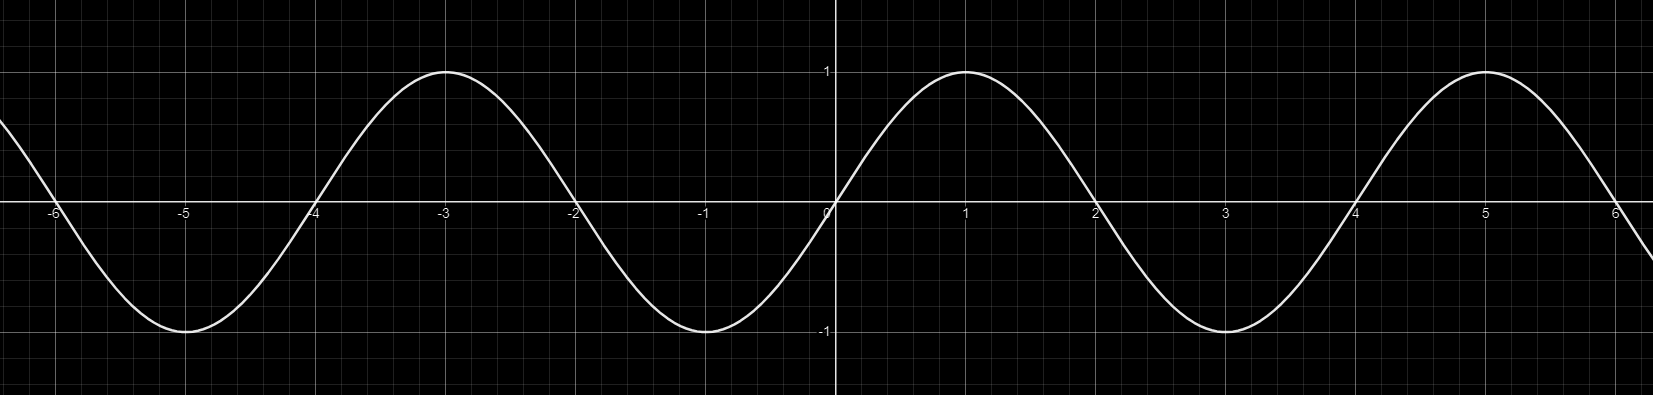
\includegraphics[scale=0.305]{graphs/2D_Real_New/FigureA}
\end{align*}
\hspace{21mm}\caption{Figure 1: Plot of $f_2(x)$ without scaling coefficients on the interval $-6 < x < 6$}

\begin{align*}
  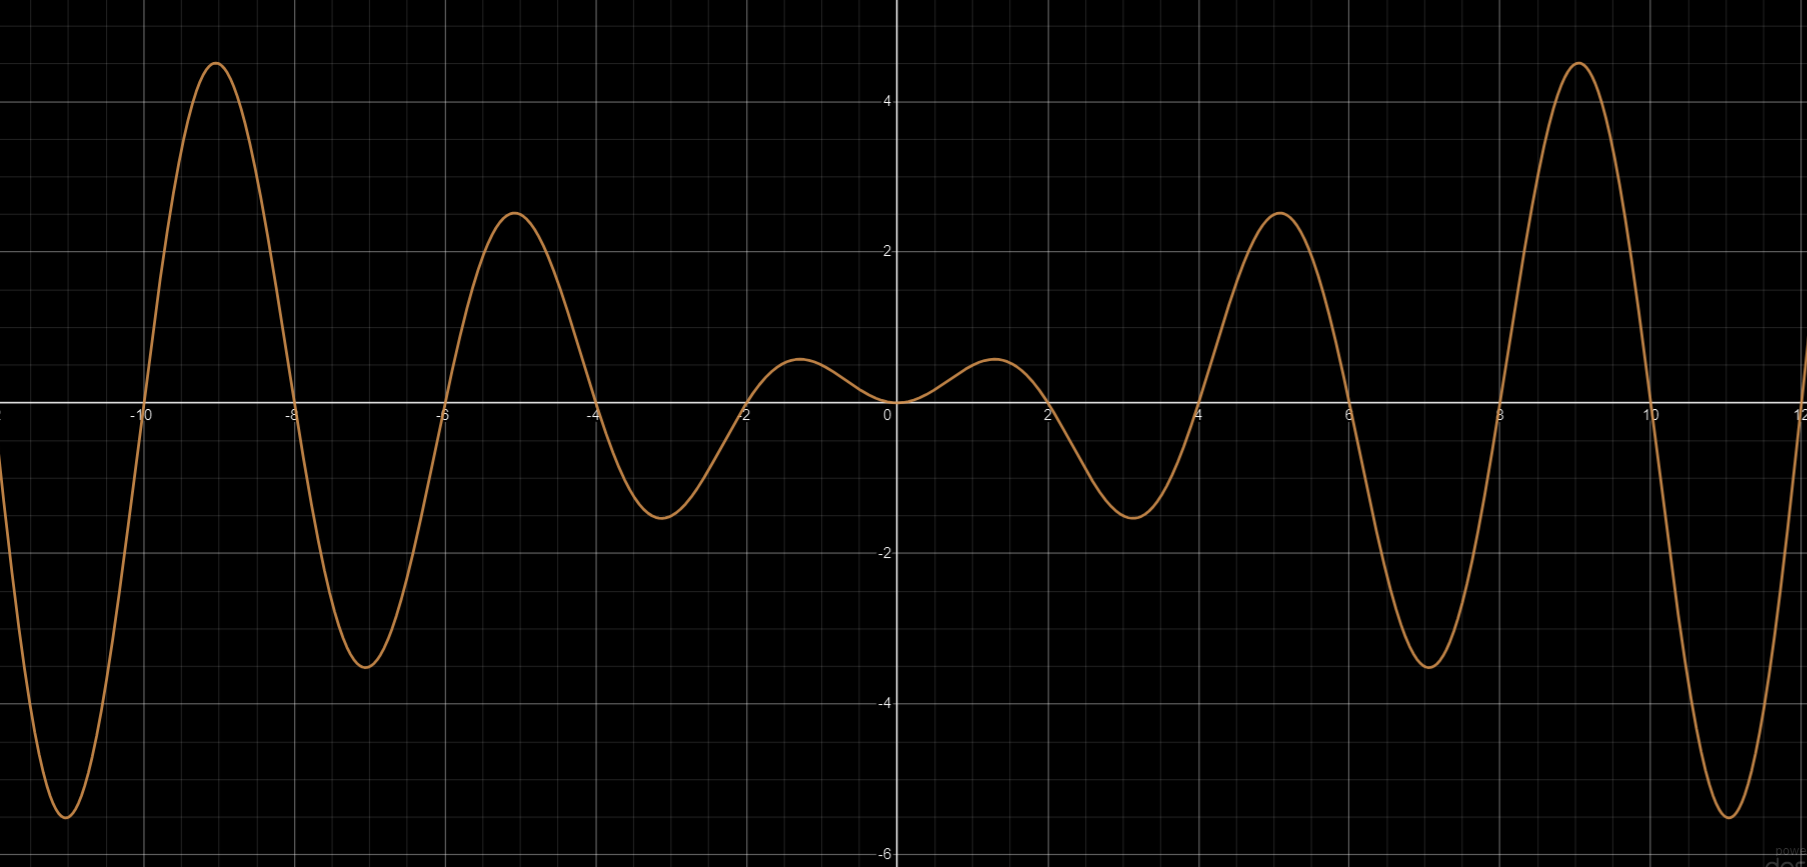
\includegraphics[scale=0.28]{graphs/2D_Real_New/Figure1_2}
\end{align*}
\hspace{21mm}\caption{Figure 2: Plot of $f_2(x)$ with scaling coefficients on the interval $-13 < x < 13$}

The two desired properties of an $a_k(x)$ function are (1) its amplitude is equal to $\alpha \frac{x}{k}$ and (2) its zeros are integer multiples of k.
Now, iterating this process, we will create an $a_k(x)$ for each whole number like so:

\begin{align*}
	a_2(x) = |\alpha \frac{x}{2}\sin\left(\frac{\pi x}{2}\right)| \\
	a_3(x) = |\alpha \frac{x}{3}\sin\left(\frac{\pi x}{3}\right)| \\
	a_4(x) = |\alpha \frac{x}{4}\sin\left(\frac{\pi x}{4}\right)|	\\
	a_5(x) = |\alpha \frac{x}{5}\sin\left(\frac{\pi x}{5}\right)| \\
	a_6(x) = |\alpha \frac{x}{6}\sin\left(\frac{\pi x}{6}\right)|	\\
	...
\end{align*}

Now plotting an $a_k(x)$ function for every whole number, except for 1, whose graph is shown without scaling coefficients in Figure 3, and with scaling coefficients in Figure 4.

\begin{align*}
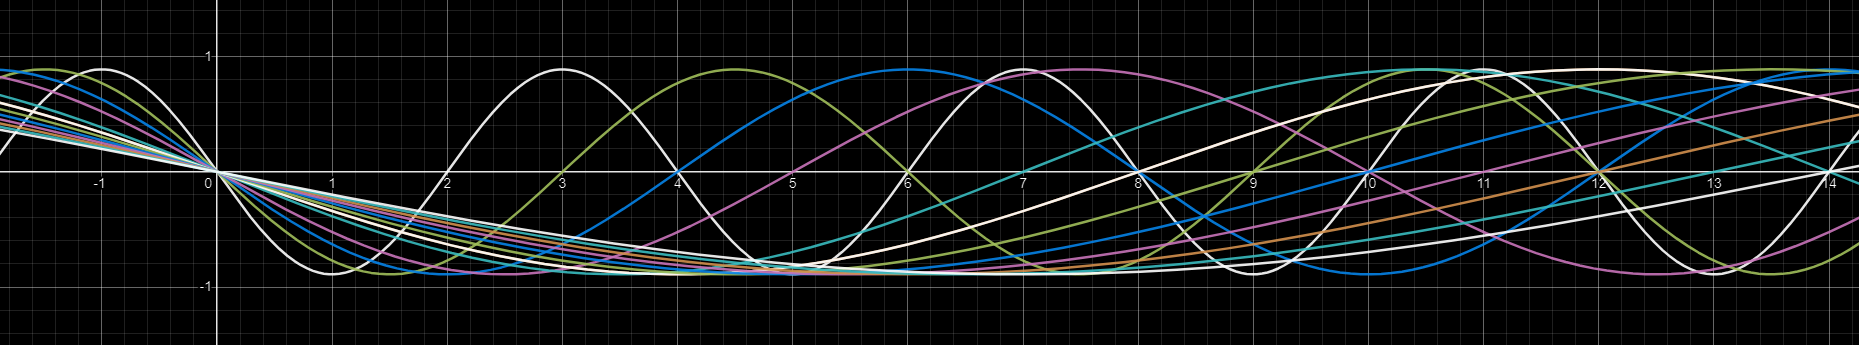
\includegraphics[scale=0.31]{graphs/2D_Real_New/FigureB_redone}
\end{align*}
\hspace{15mm}\caption{Figure 3: Graph of the Sieve of Eratosthenes, without Scaling}

\begin{align*}
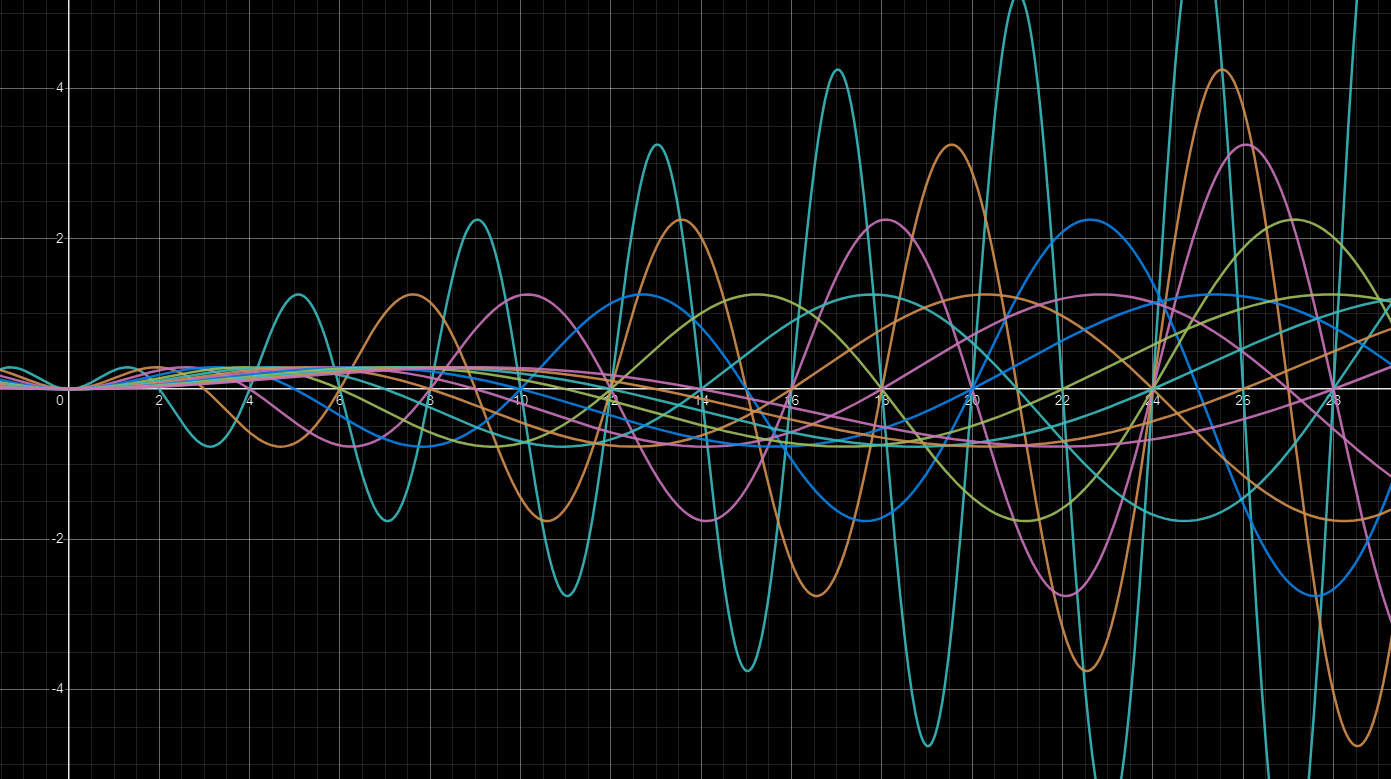
\includegraphics[scale=0.33]{graphs/2D_Real_New/Figure4_redone}
\end{align*}
\hspace{15mm}\caption{Figure 4: Graph of the Sieve of Eratosthenes, with Scaling} \\

By doing this, we have essentially created the Sieve of Eratosthenes using sine waves. You will notice that at each prime number there is only one $a_k(x)$ wave passing through the x axis. If we had created an $a_1(x)$ function then there would be 2 $a_k(x)$ waves passing through each prime x-intercept. “A prime is only divisible by itself, and one.” Because we reject $a_1(x)$ and go straight to $a_2(x)$, this means the wave passing through any prime x-intercept is the $a_p(x)$ where P is that prime number. I.e., $a_2(x)$, $a_3(x)$, $a_5(x)$, $a_7(x)$, $a_1_1(x)$, $a_1_3(x)$, etc. \\
\newline
Now that we have created an infinite number of waves, each representing a different possible divisor, we can combine them into one wave function which has attributes from each divisor wave. We do this by using an Infinite Product to define our set of infinitely many waves. Refer to the function a(z) in the next section.

\subsection*{II. Product of sine defined as a(z)}
In this paper, we will analyze several special functions using divisor waves and extreme operators. Specifically, we will consider the functions $a(z)$, $b(z)$, $c(z)$, $d(z)$, $e(z)$, $f(z)$, $g(z)$, $h(z)$, $i(z)$, $j(z)$, $k(z)$, $l(z)$, $m(z)$, $n(z)$, $o(z)$, and the Riemann zeta function $\zeta(z)$. These functions are of the variable z, where $z = x + iy$, this will be important as sometimes the scaling coefficients will be changed from x, to iy, to $x*iy$, to $x + iy$, to explore many domains/dimensions. \\

We define the function $a(z)$ as follows:

\begin{align*}
	a(z) = |\prod_{k=2}^x \alpha\frac{x}{k}\sin\left(\frac{\pi z}{k}\right)|
\end{align*}

The Function a(z) is the infinite product of $sin(\pi*z/k)$ where $2 <= k <= x$. This function, is part of a family of functions, that provide a map of the prime, and composite numbers. The front term $\alpha\frac{x}{k}$ is used for scaling purposes, as this function is highly explosive in the y-direction as you move down the x-axis. The alpha is just a coefficient that has a slider ranging from $0<\alpha<2$ and is used to stretch the function as needed. \\
\newline
The absolute value operator in front ensures that this function stays above the x-axis. This has the same effect as $y=abs[sin(x)]$. On the inside of the sine function, we still have the $\pi$ coefficient but have now replaced the whole number associated with the $f_k(z)$ function with k so that we can test through an infinite number of whole numbers.
\begin{align*}
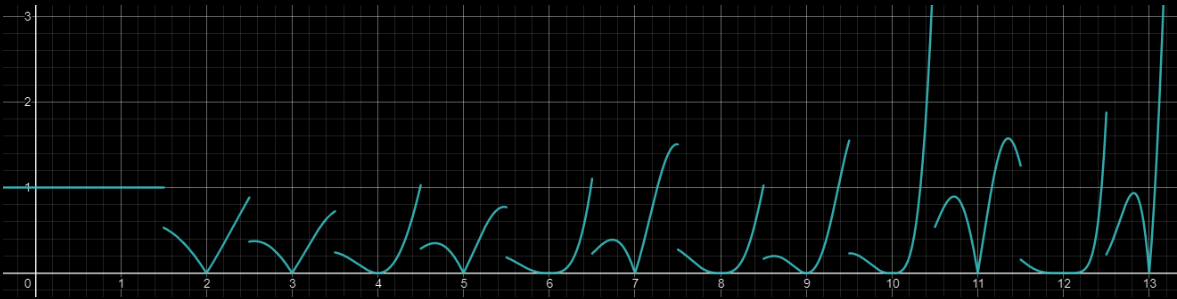
\includegraphics[scale=0.5]{graphs/2D_Real_Graphs/cuspcurve}
\end{align*}
\hspace{8mm}\caption{Figure 5: Real plot for a(x), on the interval $0 < x < 13$} \\

The Function a(x) is the infinite product of sinusoidal Divisor Waves, this essentially combines them all into one resultant wave. Looking at the graph, you can see that at each prime number there is a cusp, and at each composite number there is a curve. This is a result of the way the function approaches zero at that point. This Concept will apply to the proceeding functions as well and will allow us to analyze the continuity at each point and extract meaningful information. \\
\newline
COMPOSITE - At each composite number there are many waves all being combined at one point. For composite numbers there are more Divisor Waves that have x-intercepts causing them to trend towards zero sooner. It is because of this that a curve is created. This is even more true for highly composite numbers as highly composite numbers contain more factors. See 12 for an example of highly composite. \\
\newline
PRIME - Prime numbers do not approach zero the same way. For a prime number, there are also many waves combining at one point, but only $a_p(x)$ has an x-intercept. This means that they only reach zero for a moment before returning to larger values, and this creates the cusp.

\begin{align*}
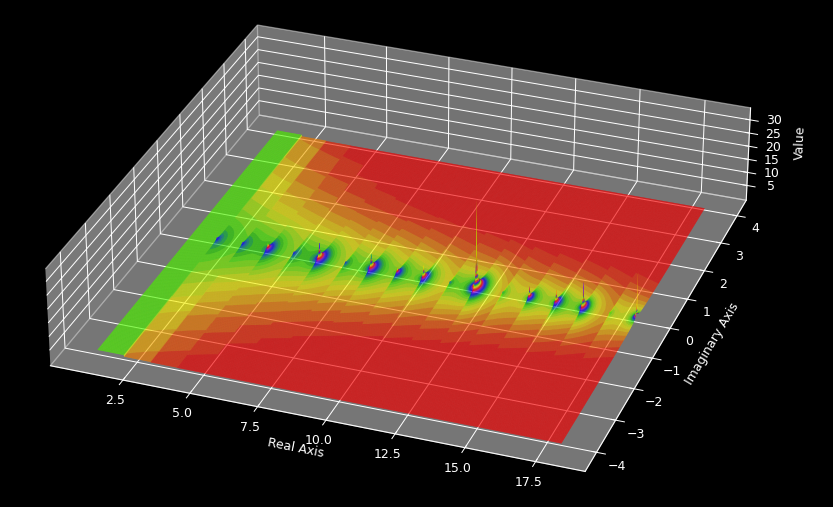
\includegraphics[scale=0.63]{graphs/3D_Complex_Graphs/product_of_sin/Complex_3D_product_of_sin_11}
\end{align*}
\hspace{15mm}\caption{Figure 6: 3D Graph of $a(x+iy)$ showcasing the zeros of the whole numbers in the complex domain on the interval of $1 < x < 18$} \\

The complex plot for a(z) reveals the same waveform with zeros at each of the whole numbers, however the composite numbers have far more distinguished peaks, as you gaze down the complex function you will see the distribution of zeros based on the distrtribution of prime and composite numbers, the peaks collecting at 8, 9, 10, 12, and 14 showcase this beautifully.
\begin{align*}
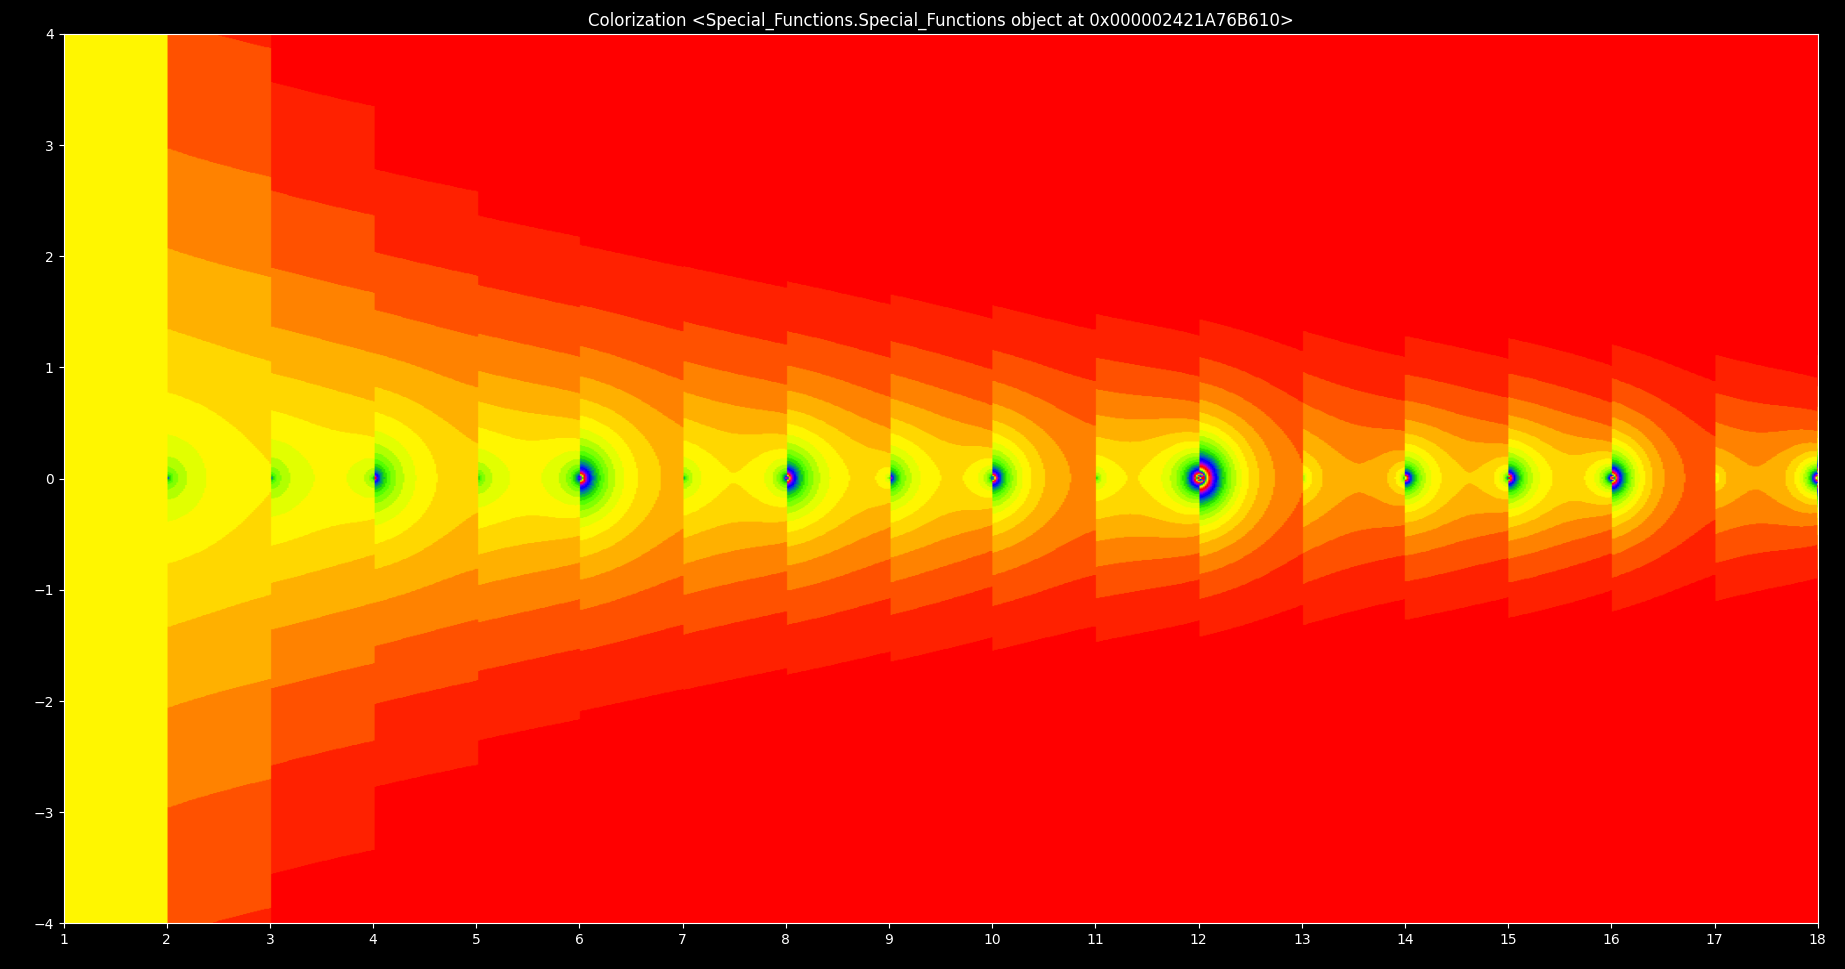
\includegraphics[scale=0.28]{graphs/3D_Complex_Graphs/product_of_sin/Complex_3D_product_of_sin_10}
\end{align*}
\hspace{8mm}\caption{Figure 7: 2D Graph of $a(x+iy)$ showcasing the zeros of the whole numbers in the complex domain on the interval of $1 < x < 18$} \\

\newpage
\subsection*{III. Initial Description of Function A(z)}
We define the Normalized a(z), function $A(z)$ as follows:
\begin{align*}
	A(z) = \frac{|\prod_{n=2}^x \alpha\frac{x}{n}\sin\left(\frac{\pi z}{n}\right)|^{-m}}{|\prod_{n=2}^x \alpha\frac{x}{n}\sin\left(\frac{\pi z}{n}\right)|^{-m}!}
\end{align*}
\begin{align*}
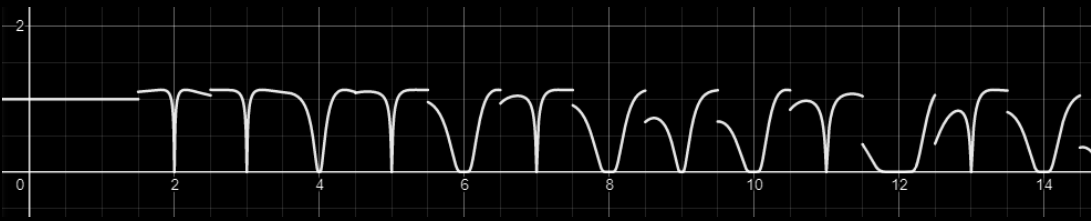
\includegraphics[scale=0.55]{graphs/2D_Real_Graphs/norm_cuspcurve}
\end{align*}
\hspace{8mm}\caption{Figure 8: 2D Graph of $A(x)$ showcasing the zeros of the real numbers} \\

This process is similar to linearization. By taking the original function a(z) and taking the fraction:
\begin{align*}
a(z)^{-m}/(a(z)^{-m})!
\end{align*} 

We are utilizing the factorial function to remove the explosive nature of a(z) and the exponent -m is a coefficient on a slider. This coefficient will allow us to magnify the function similar to $\alpha$. This actually stems from the following summation although this normalization utilizes infinite products:
\begin{align*}
\sum_{x=1}^\infty (\frac{x}{x!}) = e \rightarrow \prod_{x=1}^\infty (\frac{x}{x!}) = e^x
\end{align*}

\begin{align*}
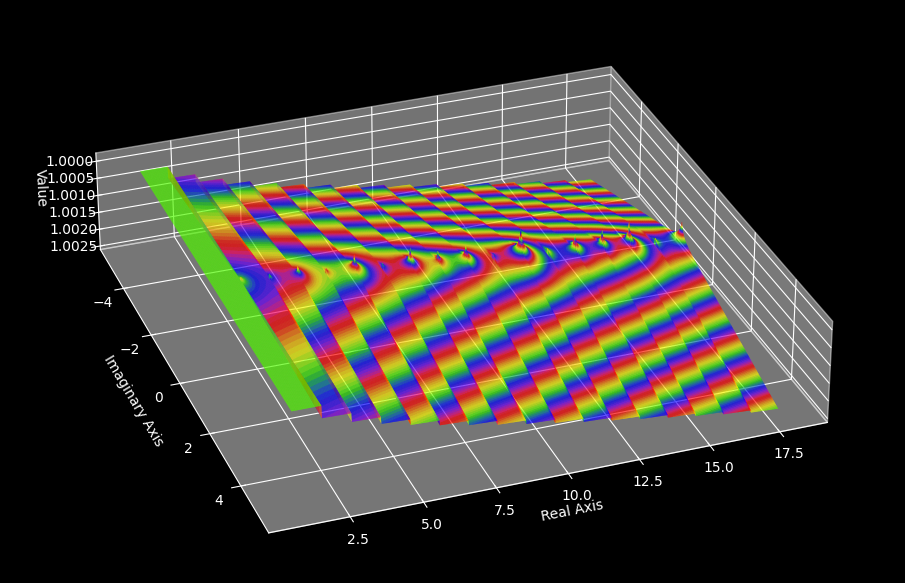
\includegraphics[scale=0.54]{graphs/3D_Complex_Graphs/product_of_sin/normalized_Complex_3D_product_of_sin_HDSET_5}
\end{align*}
\hspace{8mm}\caption{Figure 9: 3D Graph of $A(x+iy)$ showcasing the normalized zeros of the real numbers in the complex plane} \\

Similarly to Figure 6, Figure 9 showcases the complex plot for A(z) which is the normalized plot of a(z) and reveals the same waveform with zeros at each of the whole numbers, however the composite numbers have far more distinguished peaks, as you gaze down the complex function you will see the distribution of zeros based on the distribution of prime and composite numbers, the peaks collecting at 8, 9, 10, 12, and 14 showcase this beautifully.

\begin{align*}
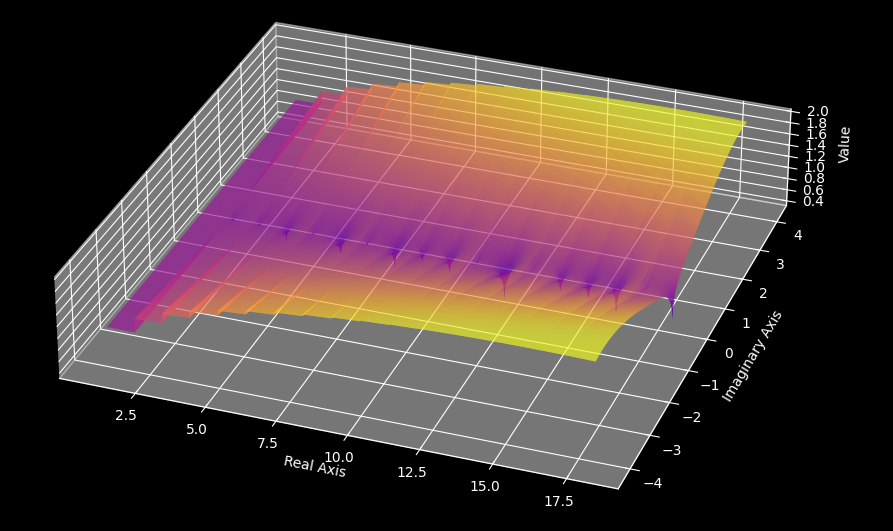
\includegraphics[scale=0.54]{graphs/3D_Complex_Graphs/product_of_sin/normalized_Complex_3D_product_of_sin_HDSET_4}
\end{align*}
\hspace{8mm}\caption{Figure 10: 3D Graph of $A(x+iy)$ showcasing the normalized zeros of the real numbers in the complex plane} \\

As you can see from the complex plots, A(z) is a function with zeros at all real numbers greater than 1, and for composite numbers contains many divisor waves which create larger peaks, or dips.

\begin{align*}
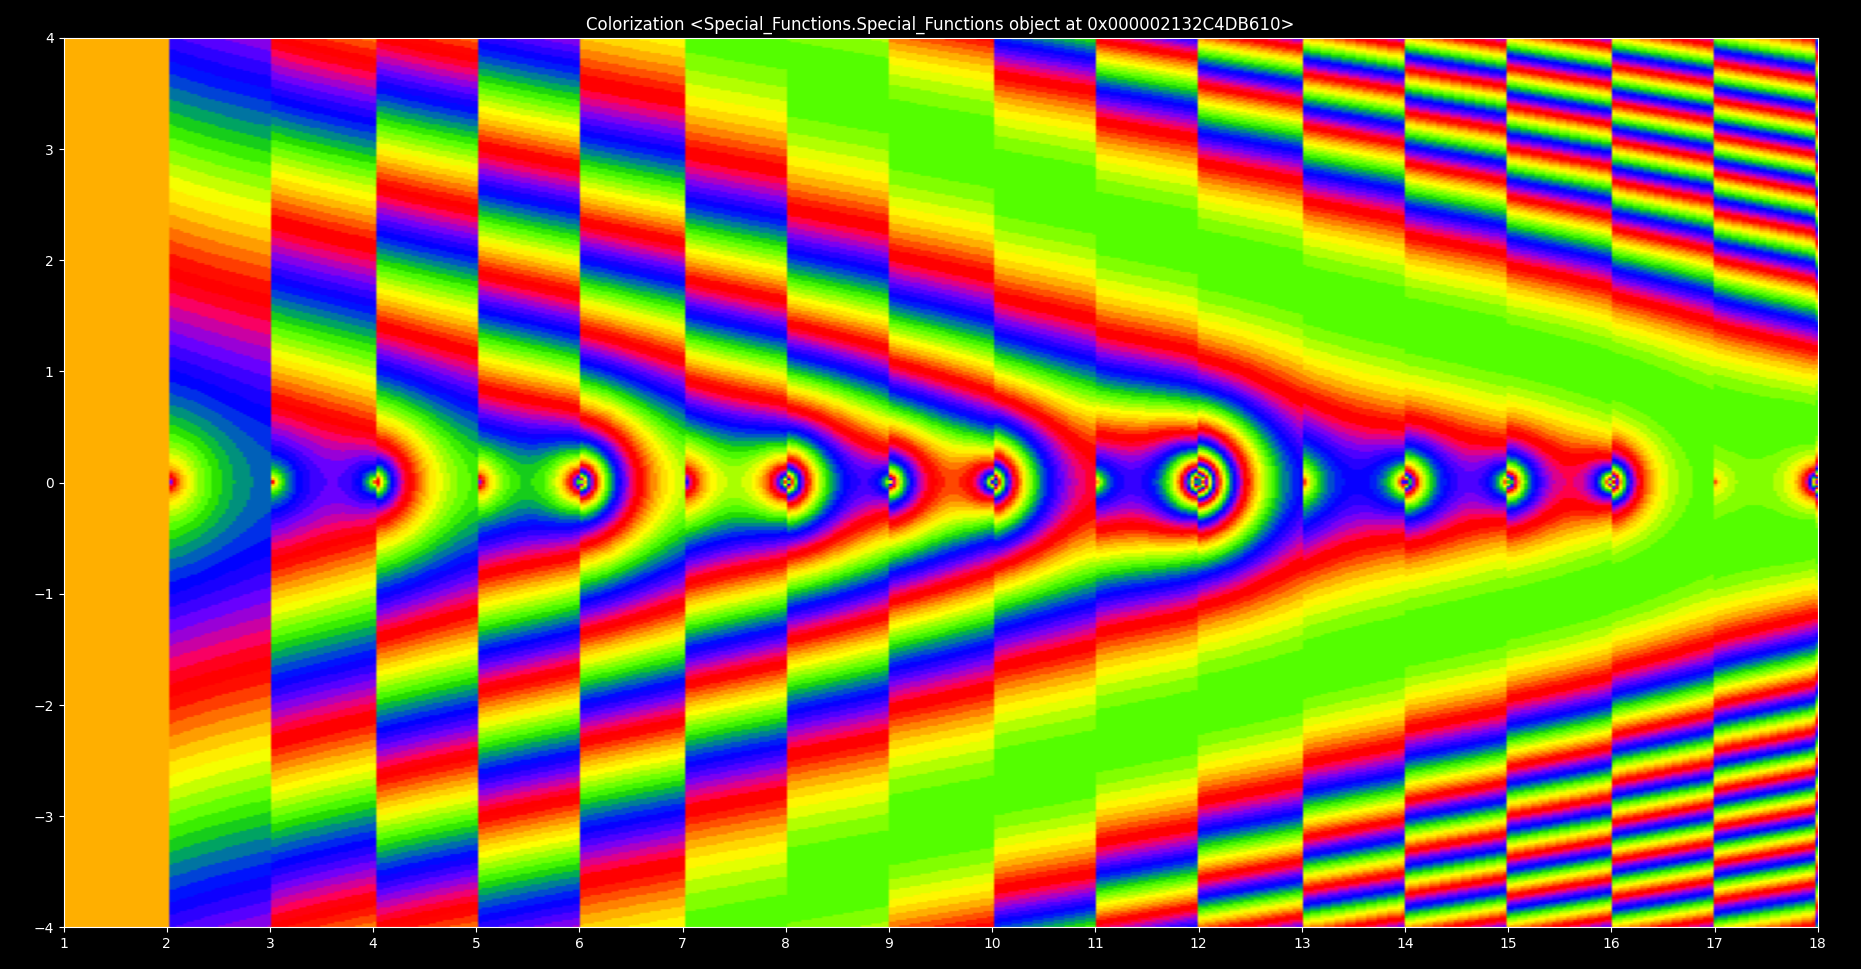
\includegraphics[scale=0.28]{graphs/3D_Complex_Graphs/product_of_sin/normalized_Complex_3D_product_of_sin_HDSET_8}
\end{align*}
\hspace{8mm}\caption{Figure 11: 2D Graph of $A(x+iy)$ showcasing the normalized zeros of the real numbers in the complex plane} \\


\newpage
\subsection*{IV. Derivation of a(z) and b(z) from the Weierstrass product formula for sin}
Derivation of a(z) and b(z) by substituting the infinite product representation of $sin(\pi*z/n)$ into the infinite product of $\sin(\pi*z/n)$: \\

We use the Weierstrass Product Formula for sin to form the relationship where k is a constant, this differs from the original Weierstrass product formula which does not contain this constant: \\
\begin{align*}
	\sin\left(\frac{\pi z}{k}\right) = \pi z\prod_{n=2}^z \left(1-\frac{z^2}{n^2k^2}\right) \\
\end{align*}

Taking the product of both sides provides function a(z) as well as the functional equation of a(z) known as b(z): \\
\begin{align*}
	\prod_{k=2}^z\sin\left(\frac{\pi z}{k}\right) = \prod_{k=2}^z \pi z\prod_{n=2}^z \left(1-\frac{z^2}{n^2k^2}\right) \\
\end{align*}

This proof shows the relationship between a(z) and b(z), and allows us to appreciate some of the beautiful relationships between these functions. The function b(z) is an equivalent form of a(z) however it has extra parameters that we can use to our advantage. \\

Now, we can expand the product out to infinity, using the expression we derived earlier:

\begin{align*}
b(x) &= \prod_{k=2}^{x} \left|\frac{\pi x}{k} \prod_{n=2}^{\infty} \left( 1 - \frac{x^2}{n^2 k^2} \right) \right| \\
&= \prod_{k=2}^{x} \left|\frac{\pi x}{k} \prod_{n=2}^{\infty} \left( 1 - \frac{x^2}{n^2 k^2} \right) \right| \\
&= \prod_{k=2}^{x} \left|\frac{\pi x}{k} \left[ \left( 1 - \frac{x^2}{(2^2)(k^2)}\right) \left( 1 - \frac{x^2}{(3^2)(k^2)}\right) \left( 1 - \frac{x^2}{(4^2)(k^2)}\right) \cdots \right]\right| \\
\end{align*}
\begin{align*}
&= \frac{\pi*x}{n}\left[ \left( 1 - \frac{x^2}{(2^2)(2^2)}\right) \left( 1 - \frac{x^2}{(2^2)(3^2)}\right) \left( 1 - \frac{x^2}{(2^2)(4^2)}\right) \cdots \right] \\
&\qquad \times \left[ \left( 1 - \frac{x^2}{(3^2)(2^2)}\right) \left( 1 - \frac{x^2}{(3^2)(3^2)}\right) \left( 1 - \frac{x^2}{(3^2)(4^2)}\right) \cdots \right] \\
&\qquad \times \left[ \left( 1 - \frac{x^2}{(4^2)(2^2)}\right) \left( 1 - \frac{x^2}{(4^2)(3^2)}\right) \left( 1 - \frac{x^2}{(4^2)(4^2)}\right) \cdots \right] \\
&\qquad \times \cdots \\
\end{align*}

\newpage
We can now use this infinite polynomial to evaluate the composite number $x = 4$ and we can see that for the factors of 4 the terms of the polynomial go to zero. \\

\begin{flushleft*}
f(4) = \\
\end{flushleft*}

\begin{align*}
= \pi*4\left\left[ \left( 1 - \frac{4^2}{(2^2)(2^2)}\right) \left( 1 - \frac{4^2}{(2^2)(3^2)}\right) \left( 1 - \frac{4^2}{(2^2)(4^2)}\right) \right] \\
\times \left[ \left( 1 - \frac{4^2}{(3^2)(2^2)}\right) \left( 1 - \frac{4^2}{(3^2)(3^2)}\right) \left( 1 - \frac{4^2}{(3^2)(4^2)}\right) \right] \\
\times \left[ \left( 1 - \frac{4^2}{(4^2)(2^2)}\right) \left( 1 - \frac{4^2}{(4^2)(3^2)}\right) \left( 1 - \frac{4^2}{(4^2)(4^2)}\right) \right] \\
= \pi*4\left\left[ \left( 1 - \frac{16}{(4)(4)}\right) \left( 1 - \frac{16}{(16)(9)}\right) \left( 1 - \frac{16}{(4)(16)}\right) \right] \\
\times \left[ \left( 1 - \frac{16}{(9)(4)}\right) \left( 1 - \frac{16}{(9)(9)}\right) \left( 1 - \frac{16}{(9)(16)}\right) \right] \\
\times \left[ \left( 1 - \frac{16}{(16)(4)}\right) \left( 1 - \frac{16}{(16)(9)}\right) \left( 1 - \frac{16}{(16)(16)}\right) \right] \\
= \cdots \left( 1 - \frac{4^2}{(2^2)(2^2)}\right) \cdots \\
= \left( 1 - \frac{4^2}{(4)(4)}\right) = 0 \\
\end{align*}

For completeness we will also evaluate the prime number $x = 3$ and we can see that when checking the factors of 3 none of the terms go to zero. \\

\begin{flushleft*}
f(3) = \\
\end{flushleft*}

\begin{align*}
= \pi*3\left\left[ \left( 1 - \frac{3^2}{(2^2)(2^2)}\right) \left( 1 - \frac{3^2}{(2^2)(3^2)}\right)  \right] \\
\times \left[ \left( 1 - \frac{3^2}{(3^2)(2^2)}\right) \left( 1 - \frac{3^2}{(3^2)(3^2)}\right)  \right] \\
= \pi*3\left\left[ \left( 1 - \frac{3^2}{(4)(4)}\right) \left( 1 - \frac{3^2}{(4)(9)}\right)  \right] \\
\times \left[ \left( 1 - \frac{3^2}{(9)(4)}\right) \left( 1 - \frac{3^2}{(9)(9)}\right)  \right] \\
= \pi*3\left\left[ \left( 1 - \frac{9}{(16)}\right) \left( 1 - \frac{9}{(36)}\right)  \right] \\
\times \left[ \left( 1 - \frac{9}{(36)}\right) \left( 1 - \frac{9}{(81)}\right)  \right] \\
= \pi*3\left\left[ \left(\frac{7}{(16)}\right) \left(\frac{27}{(36)}\right)  \right] \times \left[ \left(\frac{27}{(36)}\right) \left(\frac{72}{(81)}\right)  \right] \\
\end{align*}

\newpage
\subsection*{V. Initial Description of Function b(z)}
The function $b(z)$ is defined as the infinite product of the infinite product representation of $\sin(\pi*z/n)$:
\begin{align*}
	b(z) = |\prod_{k=2}^x \left[\frac{\beta x}{k}\left({\pi z}\prod_{n=2}^x\left(1 - \frac{z^2}{n^2k^2}\right)\right)\right]|
\end{align*}
\begin{align*}
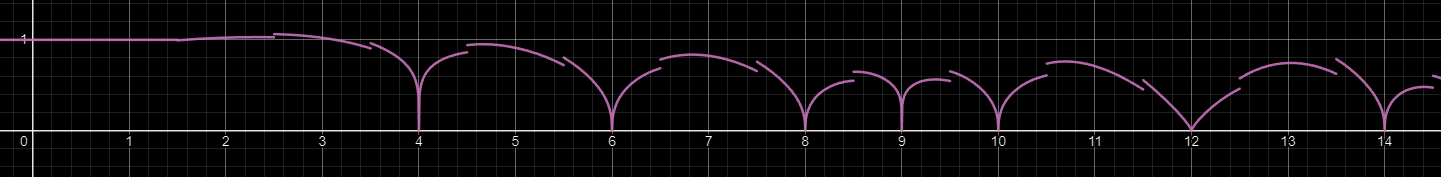
\includegraphics[scale=0.45]{graphs/2D_Real_Graphs/prime_indicator_og_redone}
\end{align*}
\hspace{8mm}\caption{Figure 12: 2D Graph of $b(x)$ showcasing the zeros of the composite numbers} \\

The Function b(x) is the infinite product of the modified product representation for sin, this essentially combines all of these modified sin waves into one resultant wave. Looking at the graph, you can see that at each prime number there is a curve, and at each composite number there is a cusp. \\
\newline
COMPOSITE - At each composite number there are many waves all being combined at one point. For composite numbers there are Divisor Waves that have x-intercepts, and in the range of primes contain no Divisor Waves going to zero, so the boundary from composite to prime causes them to trend towards zero. It is because of this that a cusp is created. Highly Composite numbers in this context actually have less of a cusp due to having more factors. See 12 for an example of highly composite. \\
\newline
PRIME - Prime numbers do not approach zero at all in this case. For a prime number, there are also many waves combining at one point, but only $b_p(x)$ has an x-intercept, and since we modified the index to be n=2 we reject the zeros with a factor of 1. This means that they never reach zero in the domain of a prime number, and this creates the non-zero curve.
\begin{align*}
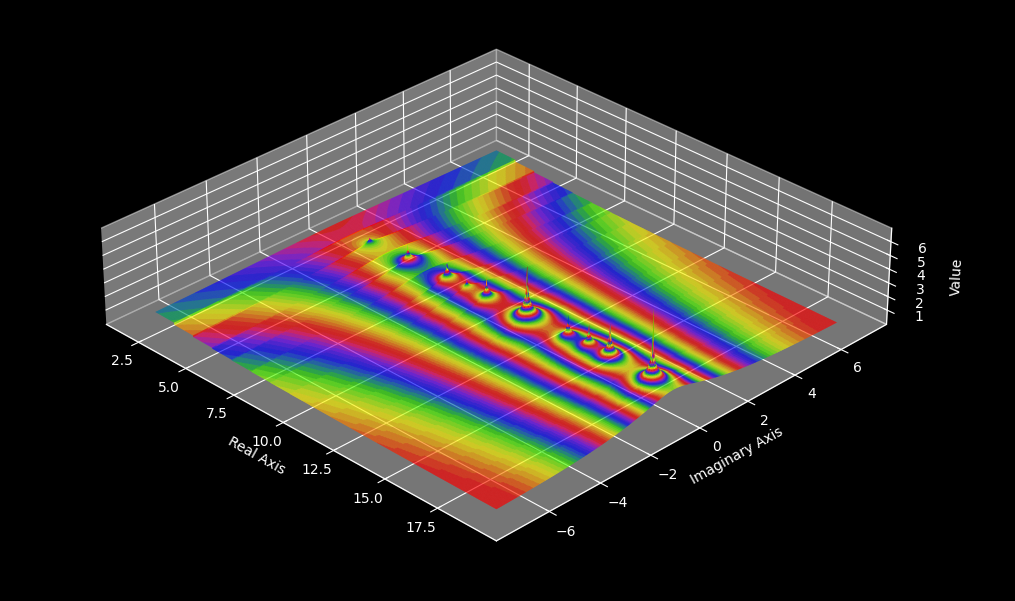
\includegraphics[scale=0.45]{graphs/3D_Complex_Graphs/product_of_product_representation_of_sin/non_normalized_goodm_prism_1}
\end{align*}
\hspace{8mm}\caption{Figure 13: 2D Graph of $b(x+iy)$ showcasing the zeros of the composite numbers} \\

We can see the zeros of $b(x + iy)$ as the blue troughs in the hills. These are the composite numbers. For each composite number there is a factor causing the product to go to zero. For all whole number values of x where x is prime, the function does not go to zero. We can observe this phenomenon at 11, and 13 on the graph as these are prime numbers. \\
\begin{align*}
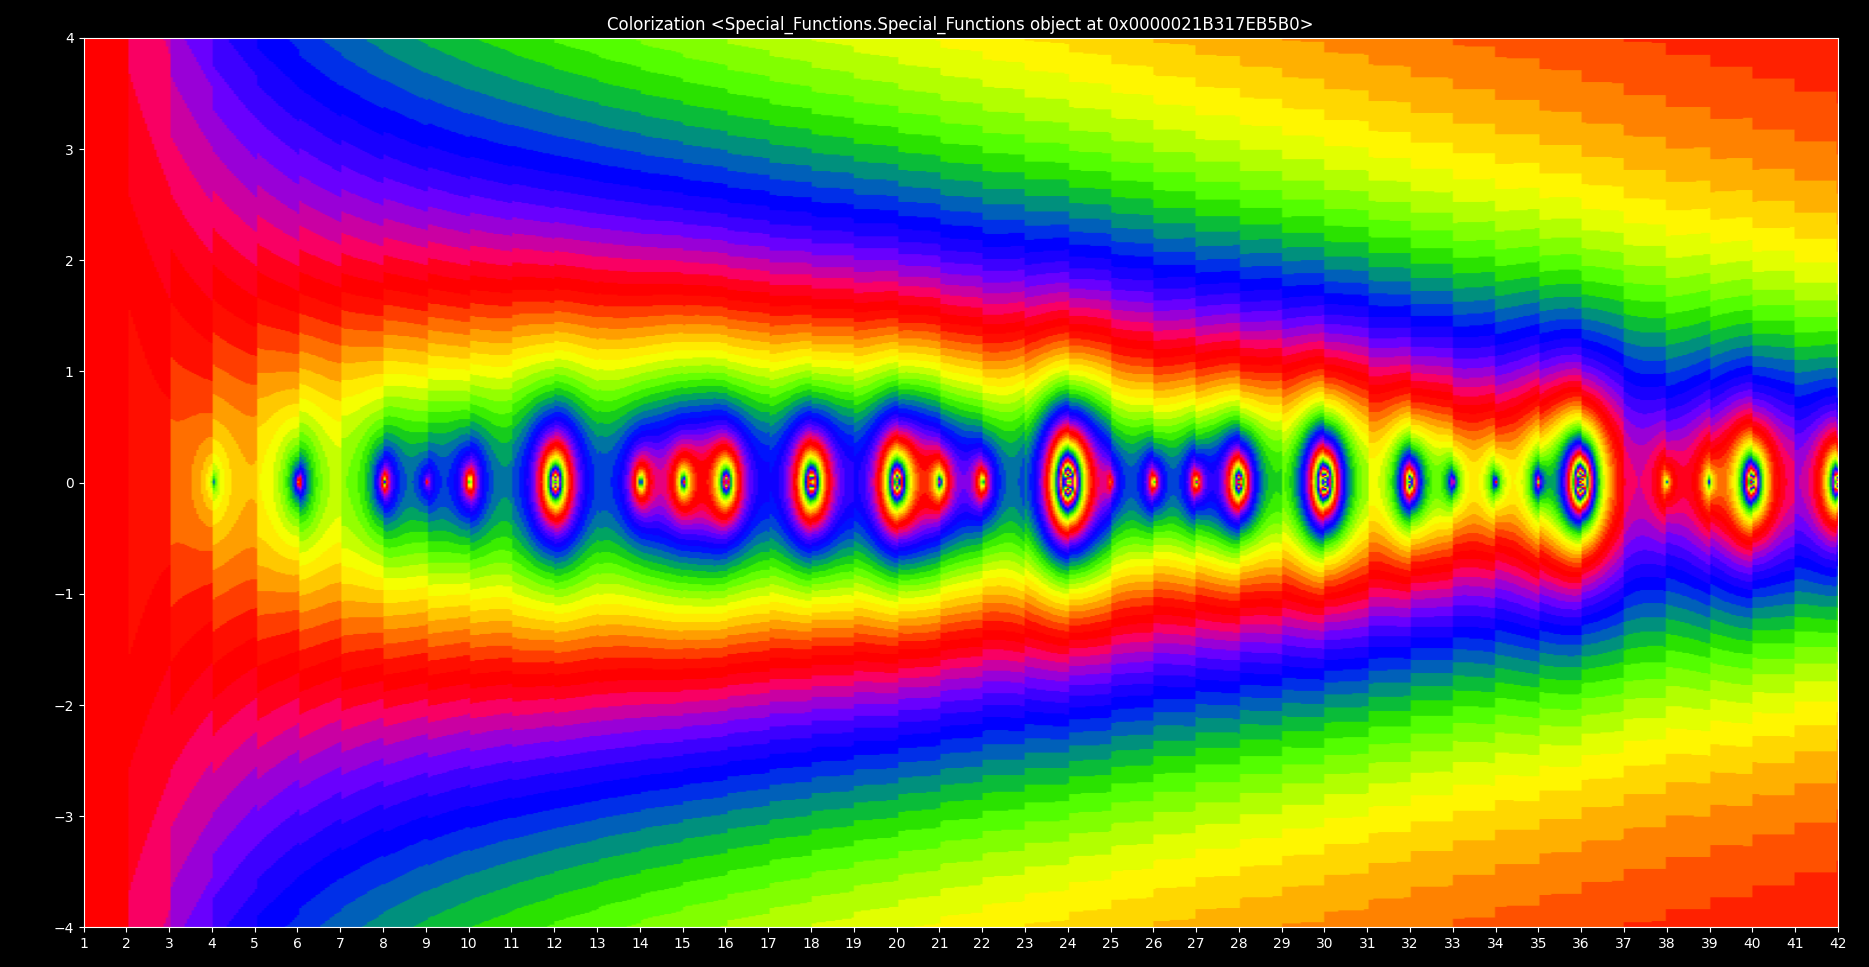
\includegraphics[scale=0.28]{graphs/3D_Complex_Graphs/product_of_product_representation_of_sin/non_normalized_goodm_prism_8}
\end{align*}
\hspace{8mm}\caption{Figure 14: 3D Graph of $b(x+iy)$ showcasing the zeros of the composite numbers} \\

The above graph is the 3D plot for $b(x+iy)$ where the 3rd dimension is height. This graph shows the complexity of the primes as it is solely dependant on the distribution of composite numbers. \\

\begin{align*}
\includegraphics[scale=0.28]{graphs/2D_Complex_Graphs/Infinite_Product_of_infinite_product_representation_of_sin/Complex_product_17_n_2-28__imaginary_scalar_logarithm}
\end{align*}
\hspace{8mm}\caption{Figure 15: 2D Fractal Colorization complex plot of $b(x+iy)$ showcasing the zeros of the composite numbers by Multipling $b(x+iy) * iy$} \\

The above fractal is the graph of b(x+iy) * iy this multiplies the function by the imaginary component, and utilized a different colorization algorithm which allows the values to stretch away from the $x-axis$ providing a beautiful fractal for the prime and composite numbers. The spikes are locations with many factors, the factors cause the function to go to infinity in the complex dimension. The prime numbers can be seen as curves between the cusps. These curves are the result of having less component waves that go to zero. \\

\newpage
\subsection*{VI. Initial Description of Function B(z)}
We define the Normalized b(z), function $B(z)$ as follows:

\begin{align*}
	B(z) = \frac{|\prod_{n=2}^x\left[\frac{\beta z}{n}\left({\pi z}\prod_{k=2}^z\left(1 - \frac{z^2}{k^2n^2}\right)\right)\right]|^{-m}}{|\prod_{n=2}^x\left[\frac{\beta z}{n}\left({\pi z}\prod_{k=2}^z\left(1 - \frac{z^2}{k^2n^2}\right)\right)\right]|^{-m}!}
\end{align*}

\begin{align*}
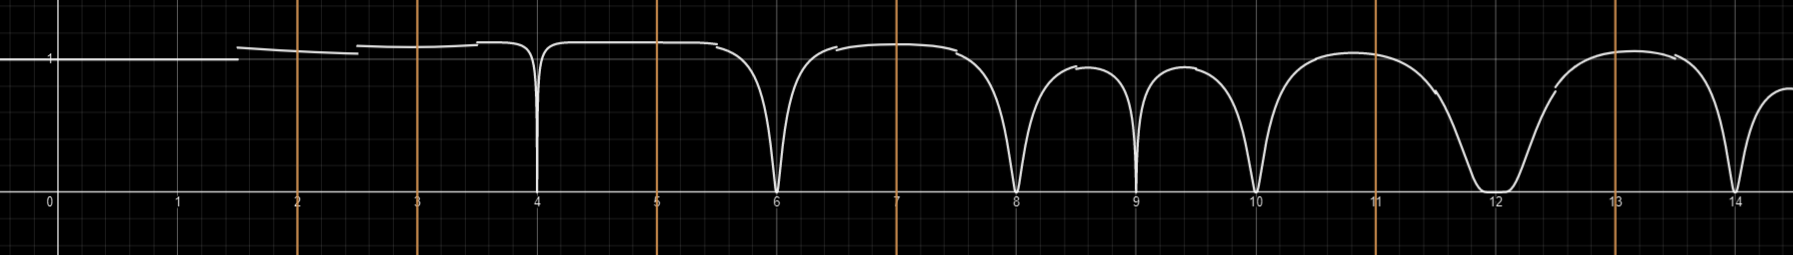
\includegraphics[scale=0.35]{graphs/2D_Real_Graphs/prime_indicator_norm}
\end{align*}
\hspace{8mm}\caption{Figure 16: 2D Graph of $B(x)$ showcasing the zeros of the composite numbers} \\

This Function is technically better than $A(z)$ as it allows us to control both of the index's n and k. By having access to n, we can have the initial value start at 2. This removes the divisor wave $B_1(x)$. Now the function no longer goes to zero at prime numbers and instead the function is greater than zero at primes and equal to zero at composites. \\

This Function is by far the most useful of the set as one could construct a piecewise function for $B(z)$ in which values of z are tested, if $B(z) > 0$, z is prime, if $B(z) = 0$, z is composite. \\

\begin{align*}
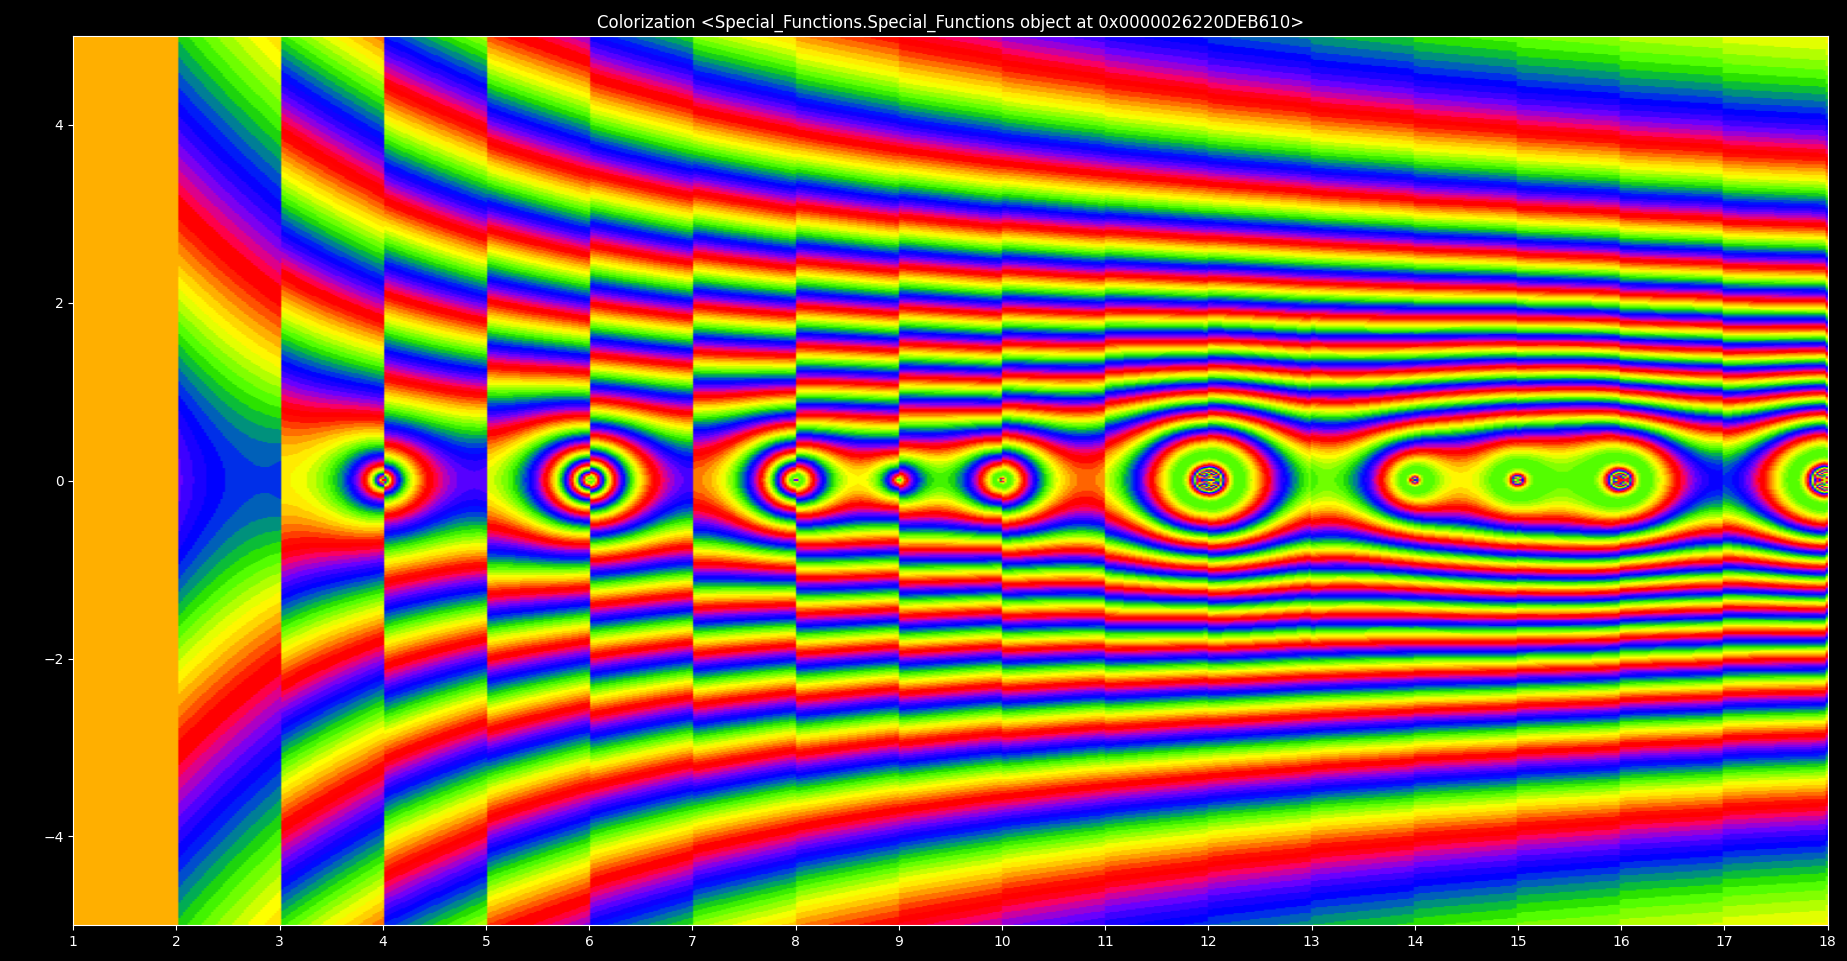
\includegraphics[scale=0.28]{graphs/3D_Complex_Graphs/product_of_product_representation_of_sin//ComplexPlot_prodprodforsin_4_Prism_Colorization_New}
\end{align*}
\hspace{8mm}\caption{Figure 17: 2D Graph of $B(x+iy)$ showcasing the zeros of the composite numbers} \\

The 2D plot of B(z) in the complex plane provides a map of the prime and composite numbers, the poles at composite numbers, versus the flat discontinuity at prime numbers show the relationship between the roots of B(z) and the composite numbers.

\begin{align*}
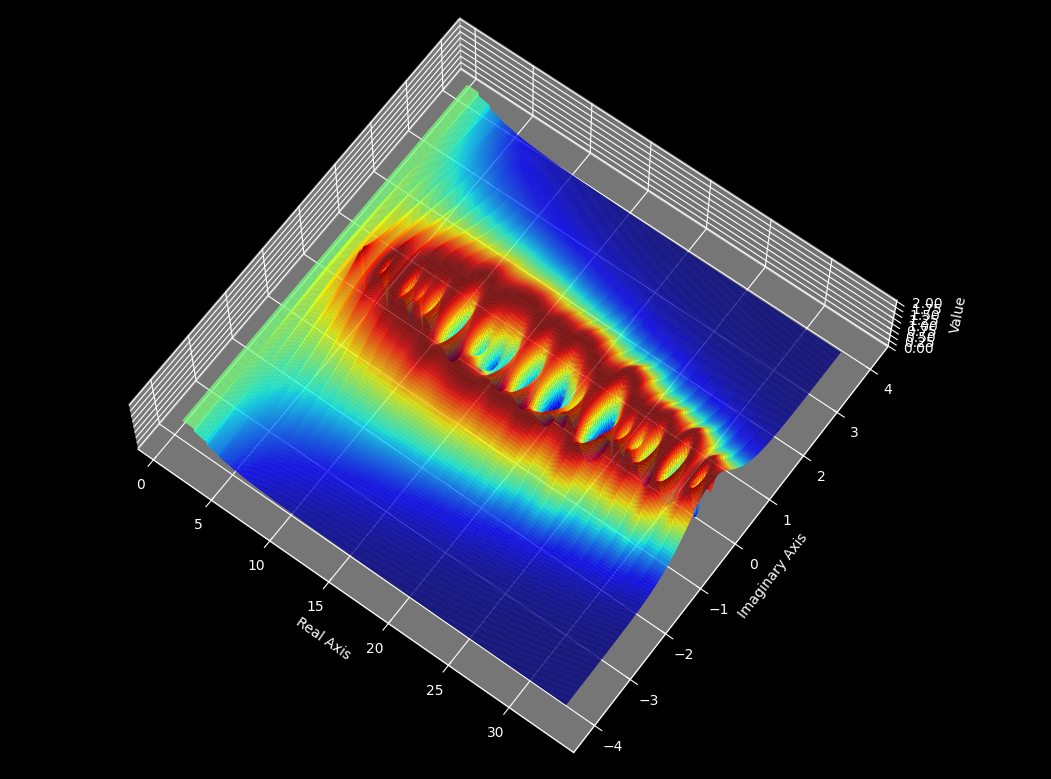
\includegraphics[scale=0.45]{graphs/3D_Complex_Graphs/product_of_product_representation_of_sin/ComplexPlot_prodprodforsin_8}
\end{align*}
\hspace{8mm}\caption{Figure 18: 3D Graph of $B(x+iy)$ showcasing the zeros of the composite numbers} \\

\begin{align*}
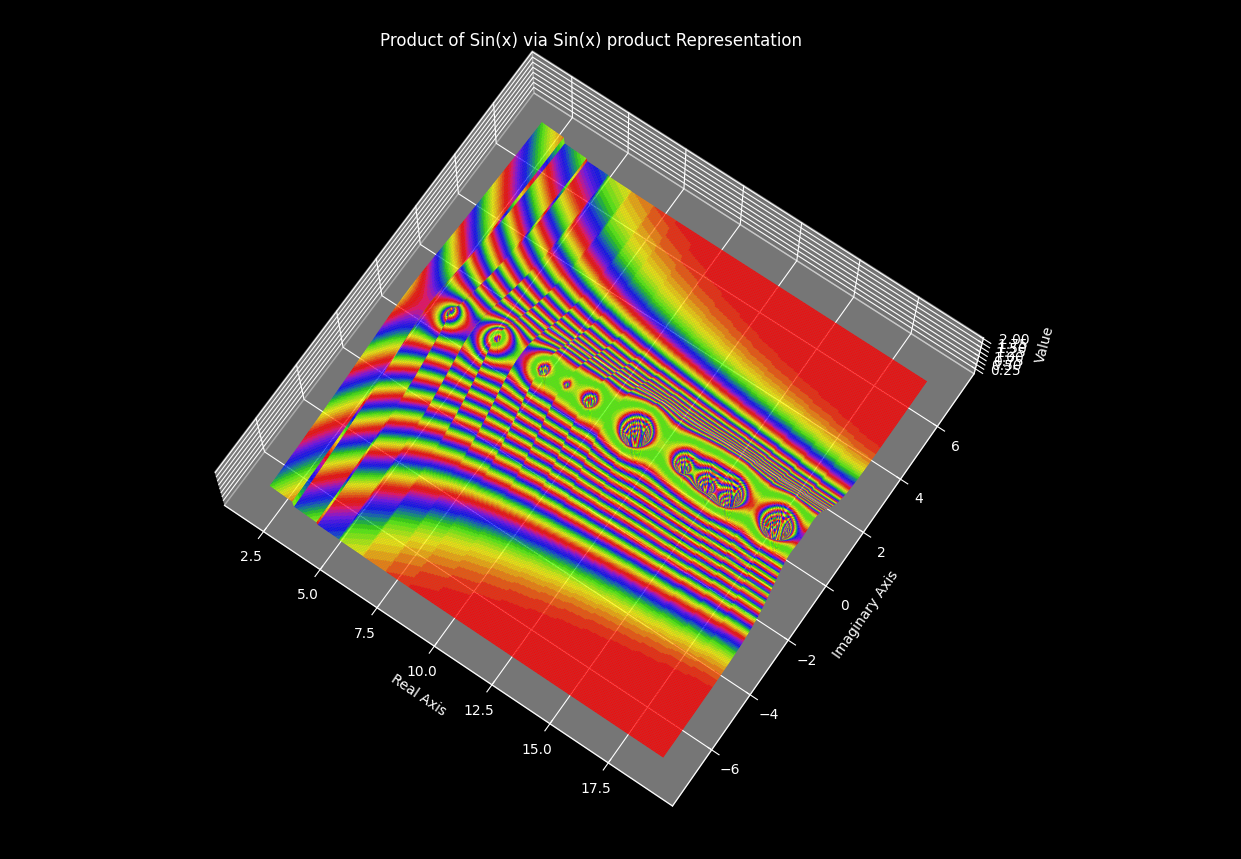
\includegraphics[scale=0.45]{graphs/3D_Complex_Graphs/product_of_product_representation_of_sin/ComplexPlot_norm_prodprodforsin_prism_3}
\end{align*}
\hspace{8mm}\caption{Figure 19: 3D Graph of $B(x+iy)$ showcasing the zeros of the composite numbers} \\

\newpage
\subsection*{VII. Exploration of a Complex Riesz Product of sin denoted as C(z)}
Due to difficulties in programming, the only complex plots presented for Riesz products will undergo Gamma function normalization as presented in Section III. We define the Normalized Complex Riesz Product of sin c(z), function $C(z)$ as follows:

\begin{align*}
	C(z) = \frac{|\prod_{n=2}^z \left(1 + |\sin\left(\pi z n\right)|\right)|^{-m}}{|\prod_{n=2}^z \left(1 + |\sin\left(\pi z n\right)|\right)|^{-m}!}
\end{align*} 

\begin{align*}
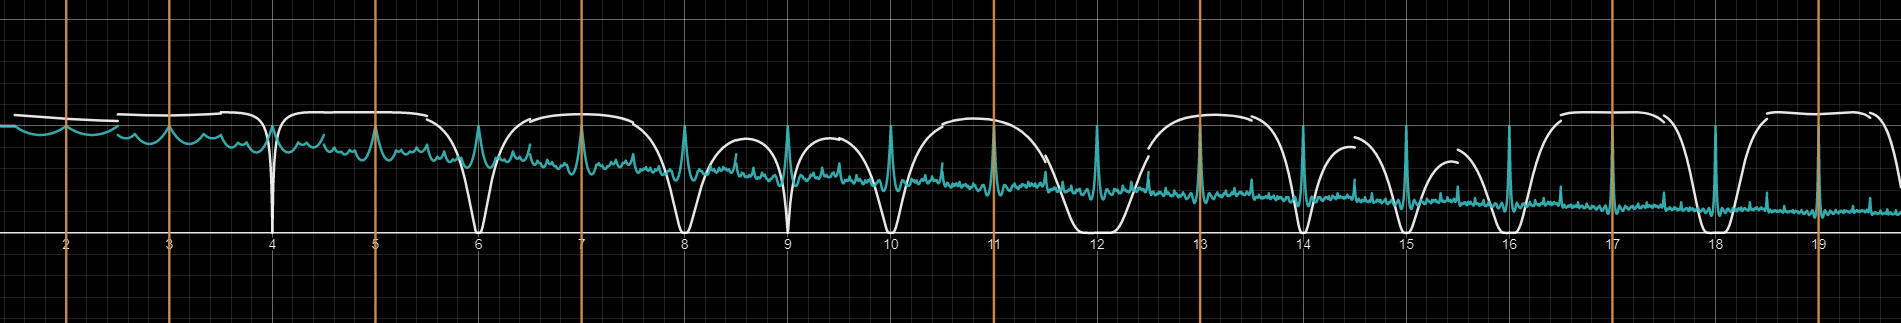
\includegraphics[scale=0.30]{graphs/2D_Real_Graphs/1+sin_prod}
\end{align*}

Figure 20: 2D Plot of C(z) overlapping with B(z) to showcase the peaks at all whole numbers for C(z).

This function's waveform has peaks at each whole number value and smaller peaks between. The number of divisions for each whole number on the real number plot in Desmos, shows a doubling of slices for each increase in index value of the product. This equation will be combined with b(z) later to create a waveform which is an indicator for prime and composite numbers while also dividing the space between whole numbers into finitely many sections as x goes to infinity.

\begin{align*}
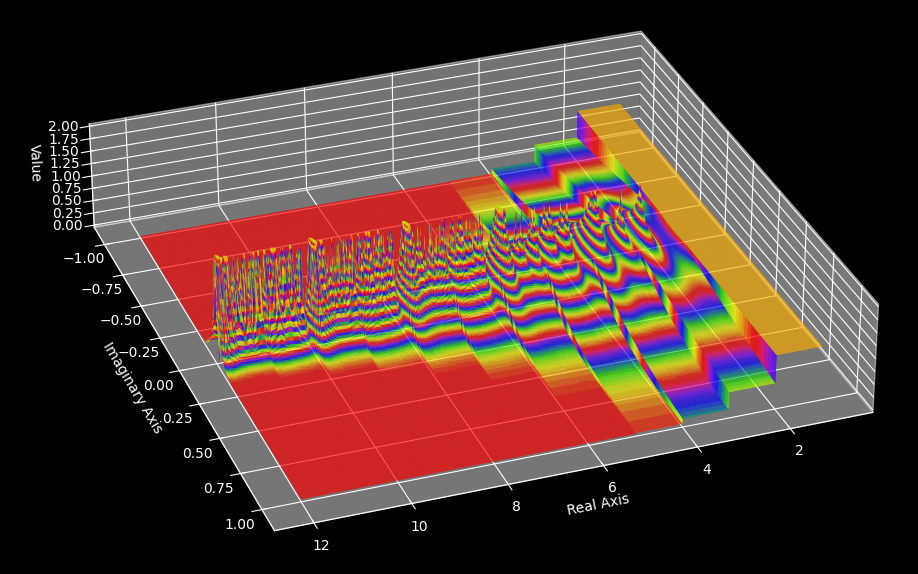
\includegraphics[scale=0.45]{graphs/3D_Complex_Graphs/riesz_sin/HD_Riesz_sin_1_12_n5}
\end{align*}
Figure 21: 3D Plot of C(z) in the complex plane to showcase the growing complexity and chaotic structure of C(z) as x increases.

This is the normalized complex plot for Riesz' infinite product of sine. The plot is fascinating as it displays poles around specific values of x, similar to Riesz cosine product, and tangent product. These poles have growing complexity in their designated regions.

\begin{figure}[ht]
\begin{minipage}[b]{0.45\textwidth}
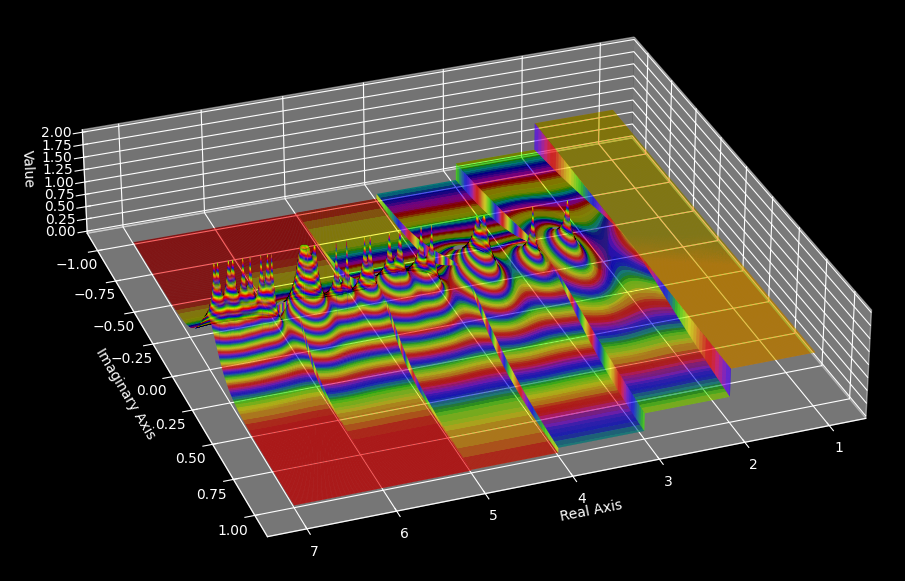
\includegraphics[scale=0.35]{graphs/3D_Complex_Graphs/riesz_sin/HD_Riesz_sin_7_12_n7}
\caption{3D Plot of C(z) in the complex plane on the interval 1 $<$ x $<$ 17}
\end{minipage}
\hfill
\begin{minipage}[b]{0.45\textwidth}
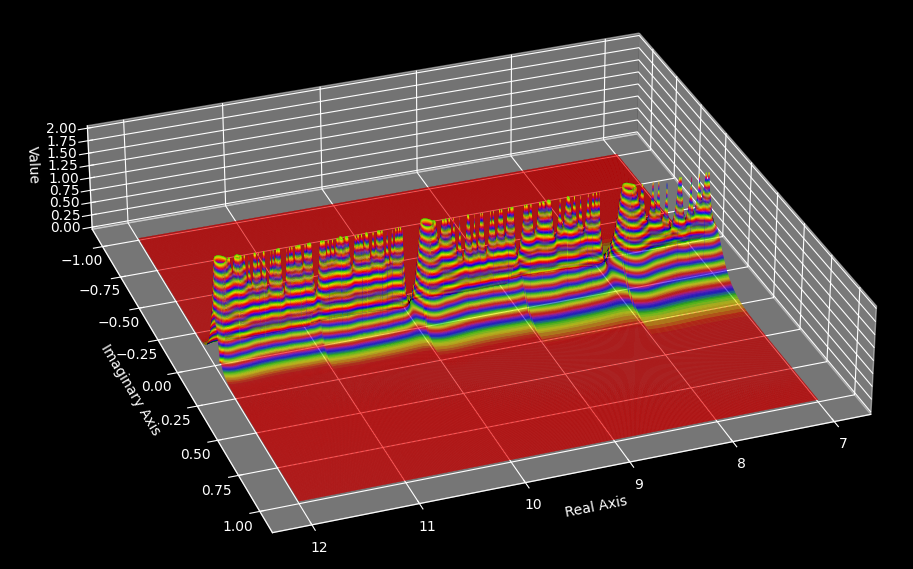
\includegraphics[scale=0.35]{graphs/3D_Complex_Graphs/riesz_sin/HD_Riesz_sin_7_12_n6}
\caption{3D Plot of C(z) in the complex plane on the interval 7 $<$ x $<$ 12}
\end{minipage}
\end{figure}

\begin{align*}
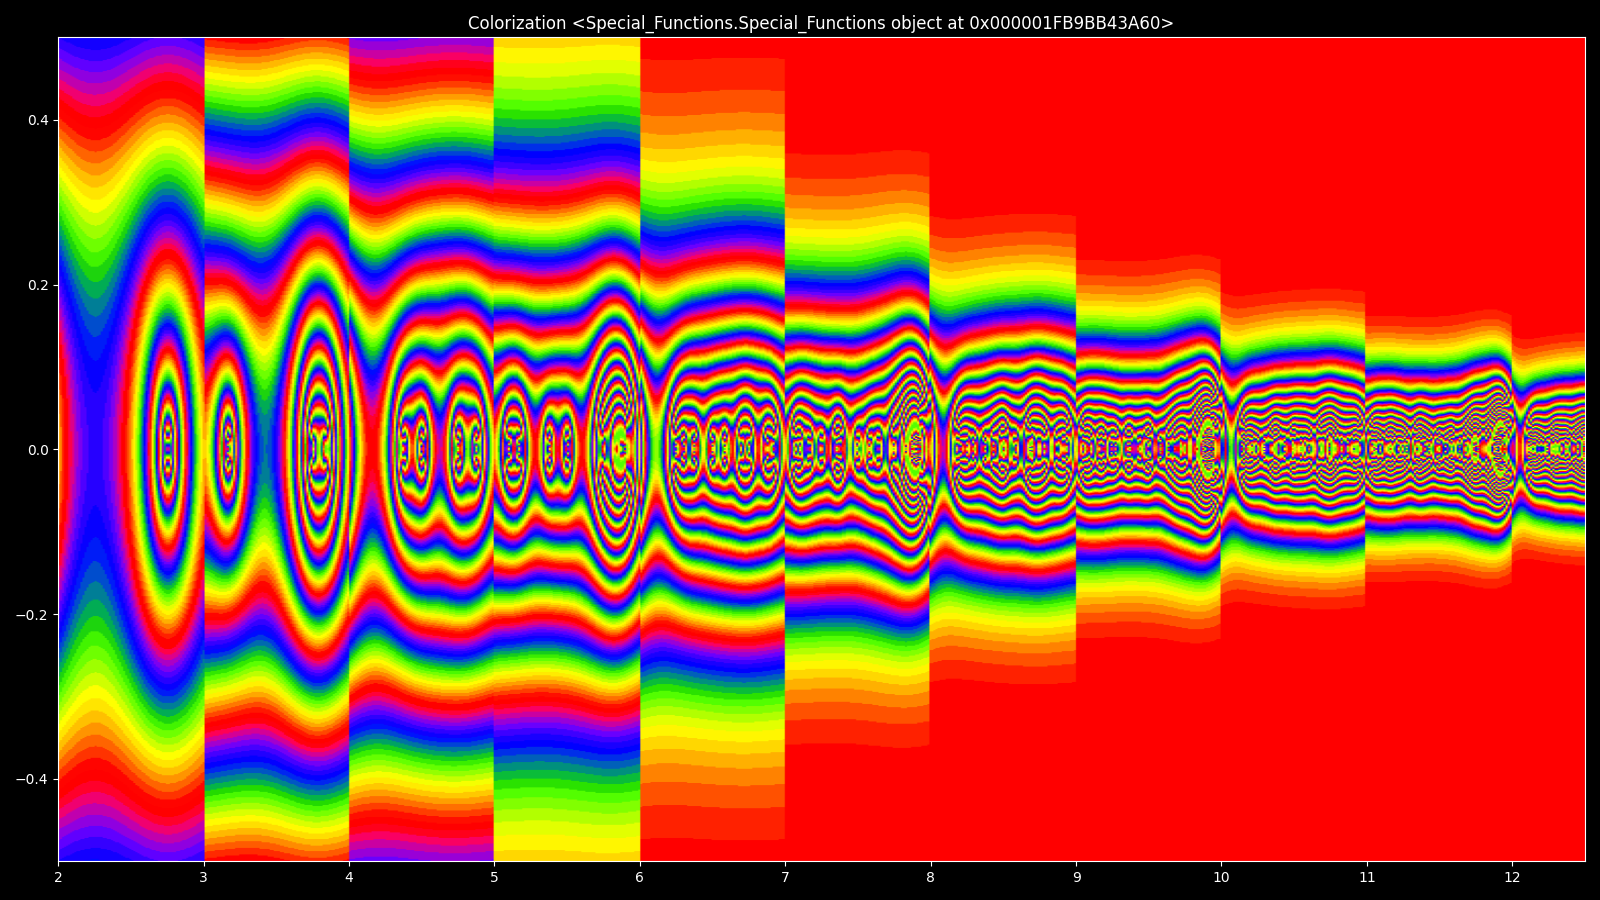
\includegraphics[scale=0.30]{graphs/3D_Complex_Graphs/riesz_sin/HD_Riesz_sin_2_12_n11}
\end{align*}
Figure 24: 2D Plot of C(z) in the complex plane on the interval 2 $<$ x $<$ 12.5

\newpage
\subsection*{VIII. Exploration of a Complex Riesz Product of cos denoted as D(z)}
Due to difficulties in programming, the only complex plots presented for Riesz products will undergo Gamma function normalization as presented in Section III. We define the Normalized Complex Riesz Product of cos d(z), function $D(z)$ as follows:
\begin{align*}
	D(z) = \frac{|\prod_{n=2}^z \left(1 + |\cos\left(\pi z n\right)|\right)|^{-m}}{|\prod_{n=2}^z \left(1 + |\cos\left(\pi z n\right)|\right)|^{-m}!}
\end{align*} 

The second factor involves an infinite product of $(1 + cos(pixn))$ over all positive integers n between 2 and x. This is a way of constructing a product of terms that oscillate between positive and negative values, with the amplitude of the oscillation increasing as n increases. The factor of pi in the cosine function reflects the periodicity of the cosine wave.

Taken together, the two products combine to create a highly complex function that is difficult to analyze in general. However, it is clear that the function involves a combination of products of terms that are close to 1 and products of oscillating terms, which suggests that the function may exhibit highly irregular behavior as x varies. \\

\begin{align*}
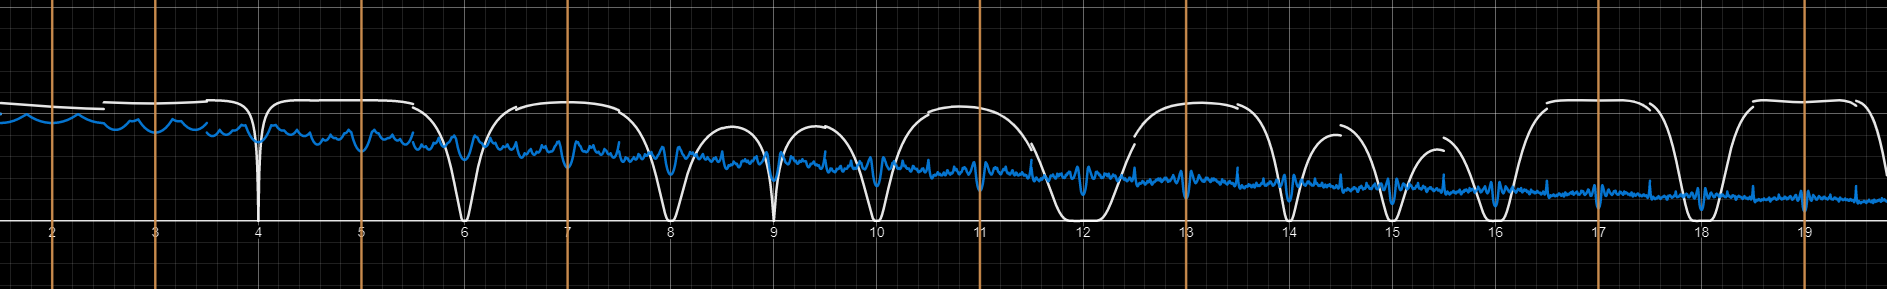
\includegraphics[scale=0.30]{graphs/2D_Real_Graphs/1+cos_prod}
\end{align*}
Figure 22: 2D Plot of D(z) overlaping with B(z) to showcase the troughs at all whole numbers for D(z).

This function's waveform has troughs at each whole number value and smaller troughs between. This equation will be combined with B(z) later to create a waveform which is an indicator for prime and composite numbers while also dividing the space between whole numbers into finitely many sections as x goes to infinity.

\begin{align*}
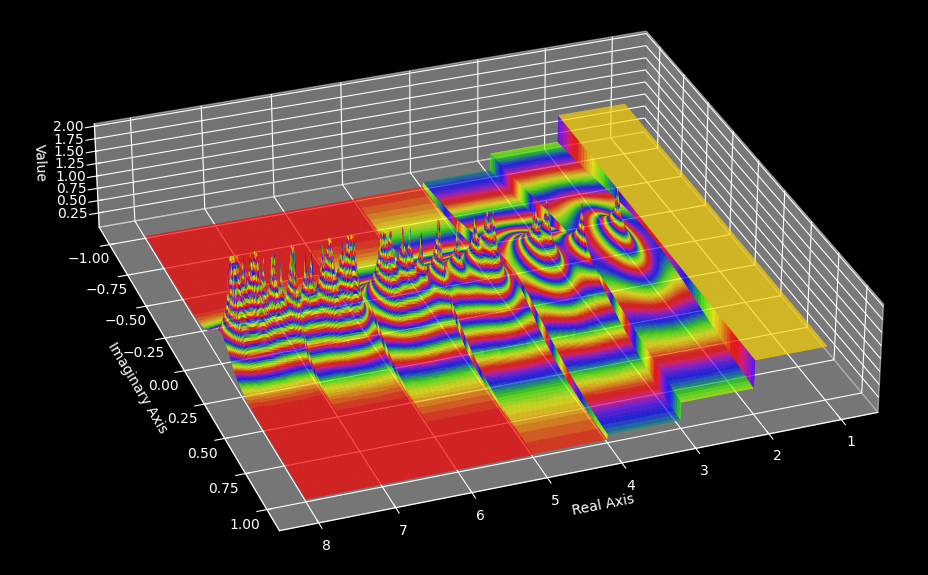
\includegraphics[scale=0.45]{graphs/3D_Complex_Graphs/riesz_cos/HD_Riesz_cos_2_12_n5}
\end{align*}
Figure 23: 3D Plot of D(z) in the complex plane to showcase the growing complexity and chaotic structure of D(z) as x increases.

This is the normalized complex plot for Riesz' infinite product of cosine. The plot is fascinating as it displays poles around specific values of x, similar to Riesz sine product, and tangent product.

\begin{align*}
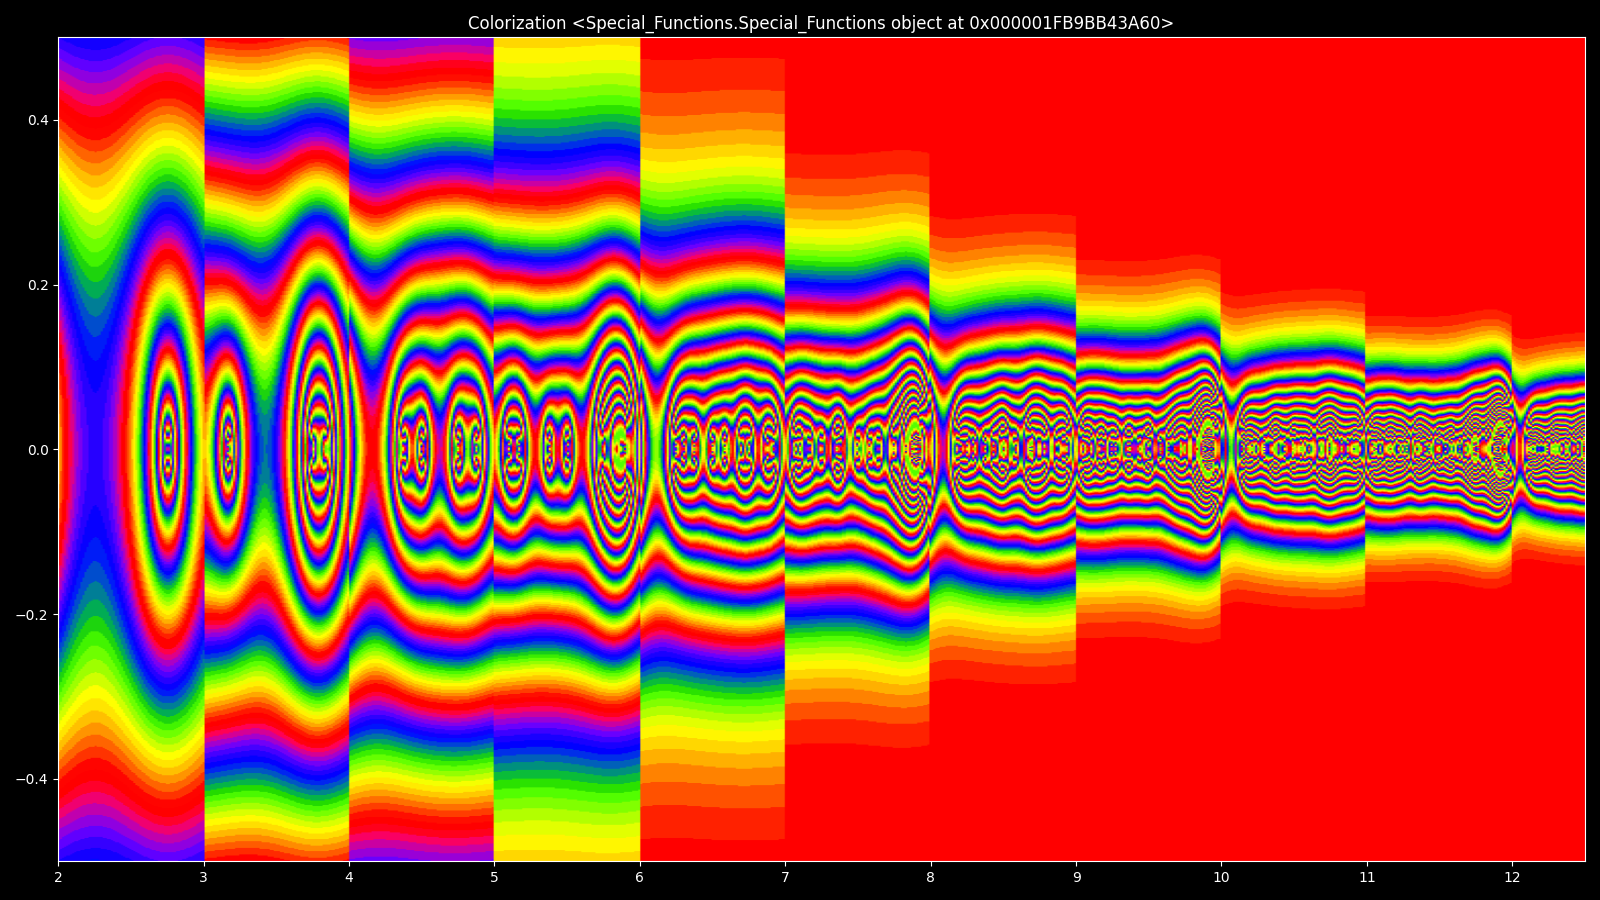
\includegraphics[scale=0.3]{graphs/3D_Complex_Graphs/riesz_cos/HD_Riesz_cos_2_12_n8}
\end{align*}
Figure 24: 3D Complex Riesz product for cos on the interval 2 $<$ x $<$ 12

\begin{align*}
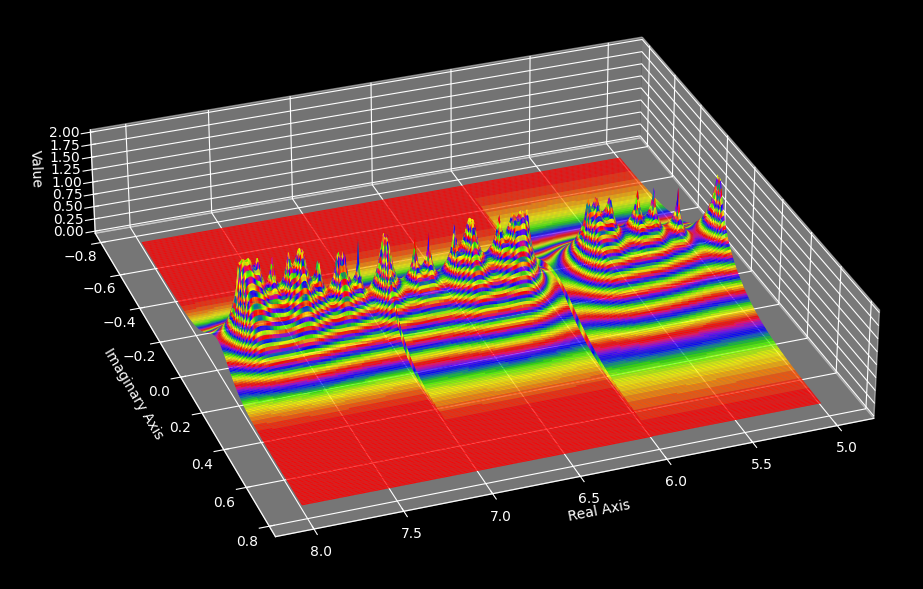
\includegraphics[scale=0.45]{graphs/3D_Complex_Graphs/riesz_cos/HD_Riesz_cos_2_12_n3}
\end{align*}
Figure 25: 3D Complex Riesz product for cos on the interval 5 $<$ x $<$ 8

\newpage
\subsection*{IX. Initial Description of Function E(z)}
We define the Normalized e(z), function $E(z)$ as follows:

\begin{align*}
	I(z) = \frac{|\prod_{n=2}^z \left(1 + |\tan\left(\pi z n\right)|\right)|^{-m}}{|\prod_{n=2}^z \left(1 + |\tan\left(\pi z n\right)|\right)|^{-m}!}
\end{align*} 

\begin{align*}
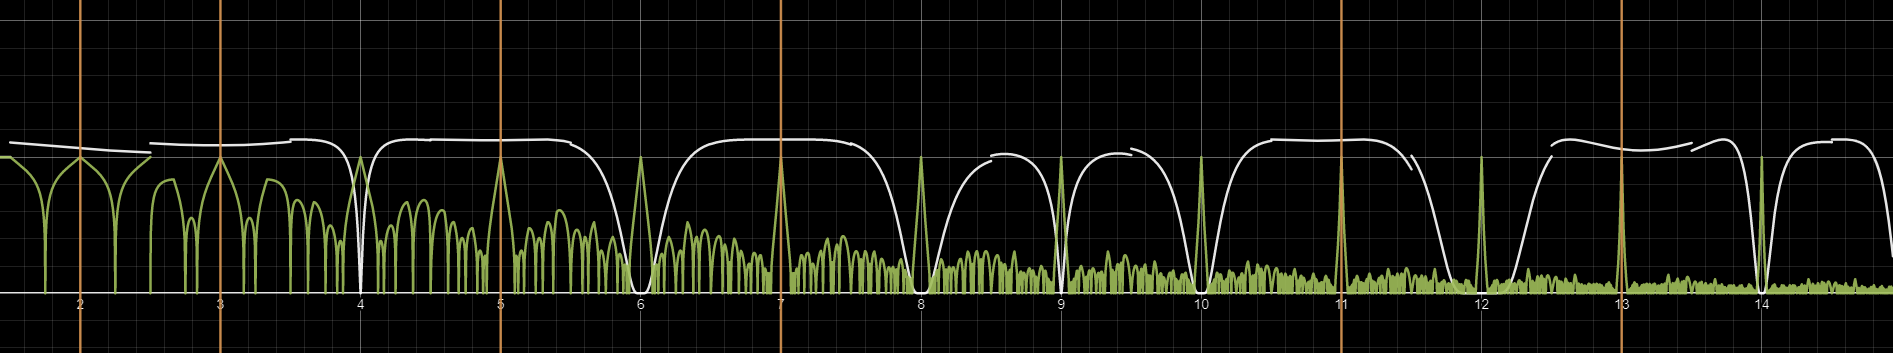
\includegraphics[scale=0.30]{graphs/2D_Real_Graphs/prod_1+tan}
\end{align*}
Figure 26: 2D Plot of E(z) overlaping with B(z) to showcase the peaks at all whole numbers for E(z).

This function's waveform has peaks at each whole number value and bumpy patches between. These sections show nicely the divisions that are taking place across the number line that section these areas into finitely many sections which increase as x goes to infinity. This equation will be combined with b(z) later to create a waveform which is an indicator for prime and composite numbers while also dividing the space between whole numbers into finitely many sections as x goes to infinity. \\

\begin{align*}
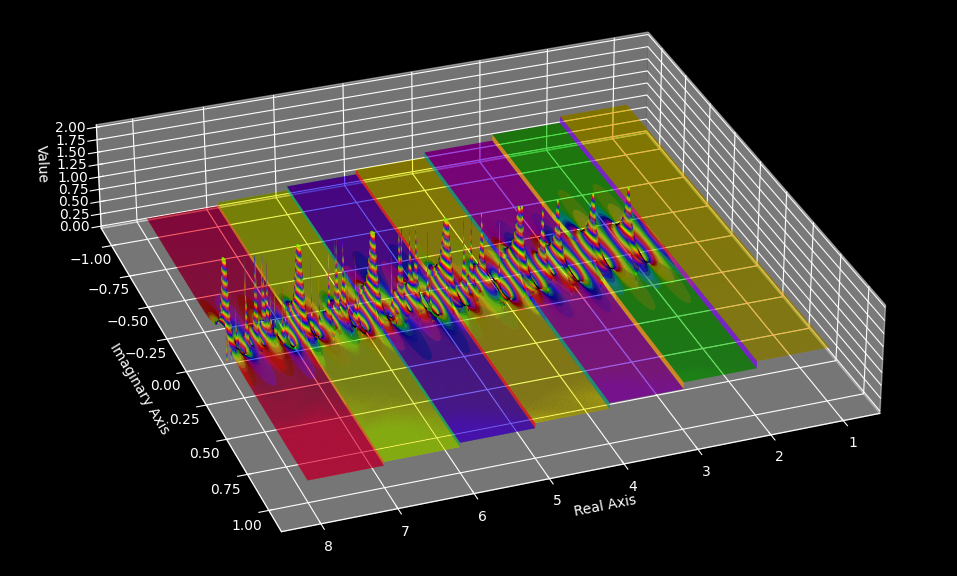
\includegraphics[scale=0.55]{graphs/3D_Complex_Graphs/riesz_tan/HD_Riesz_tan_2_12_n5}
\end{align*}
Figure 27: 3D Plot of E(z) in the complex plane to showcase the growing complexity and chaotic structure of E(z) as x increases.

This is the normalized complex plot for Riesz' infinite product of tangent. The plot is fascinating as it displays poles around specific values of x, similar to Riesz sine product, and cos product.

\begin{align*}
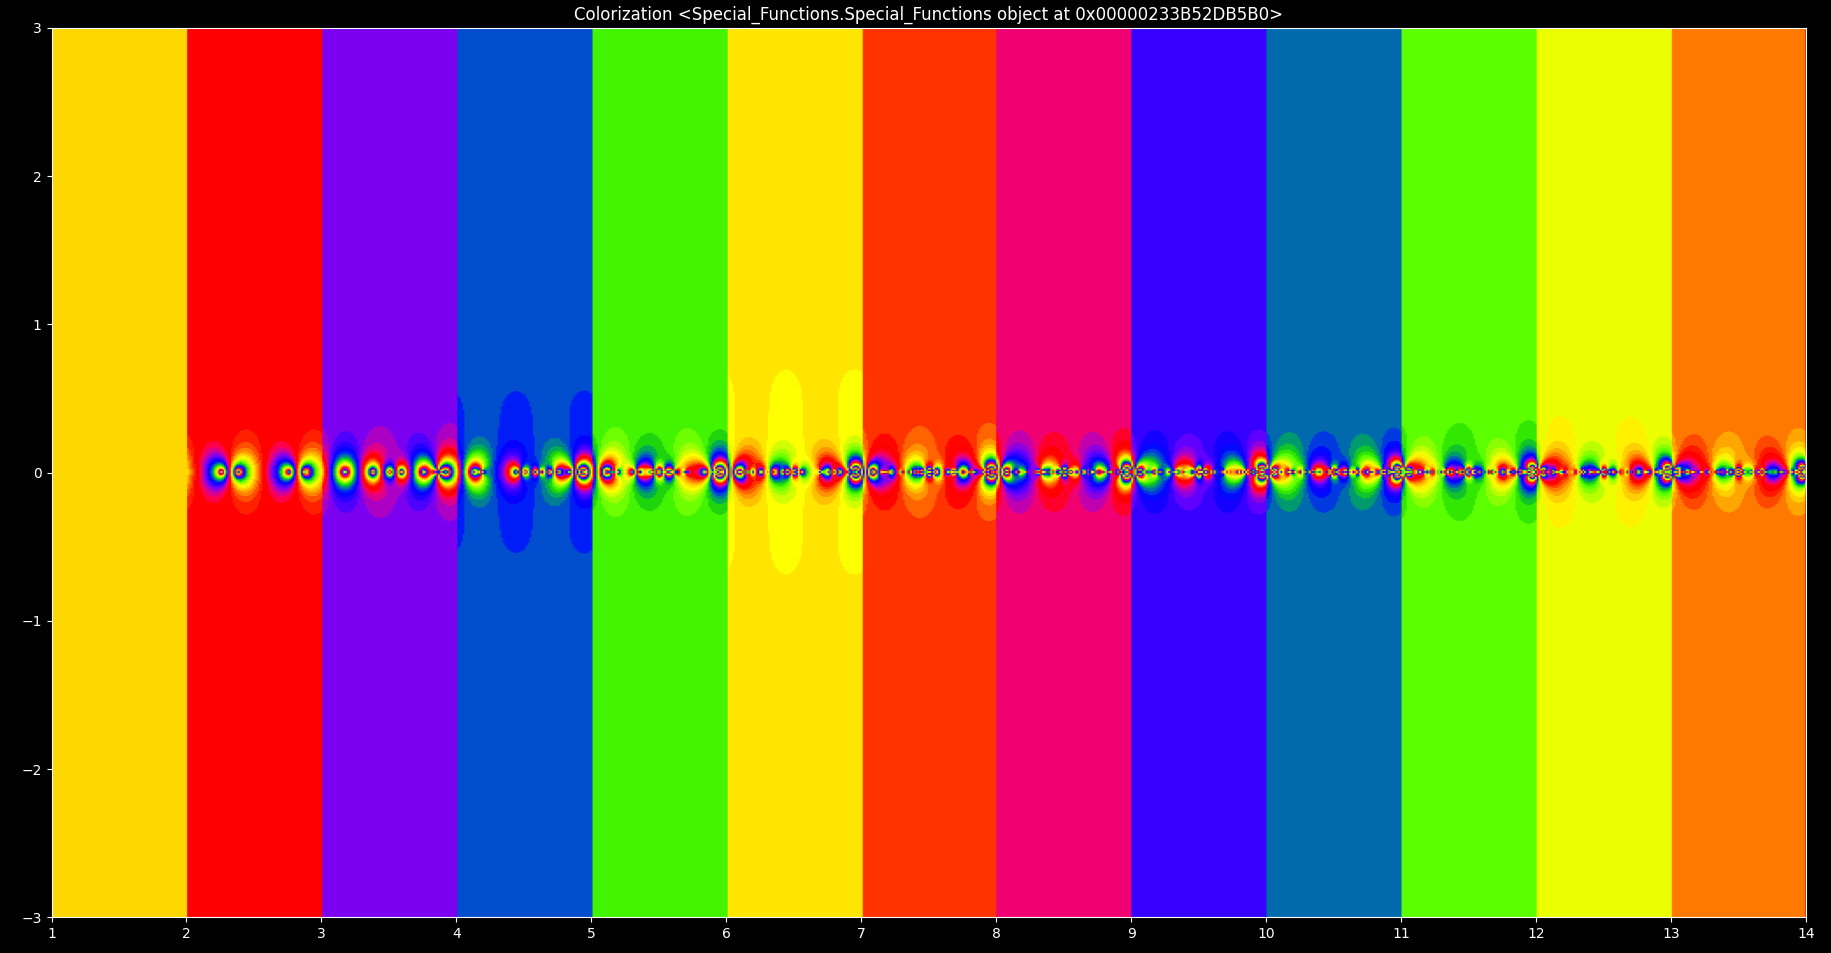
\includegraphics[scale=0.28]{graphs/3D_Complex_Graphs/riesz_tan/Ries_tan_norm_2}
\end{align*}
Figure 28: 2D Plot of E(z) in the complex plane to showcase the many zeros of E(z) each defined in their own regions with growing compplexity as x increases.

\begin{align*}
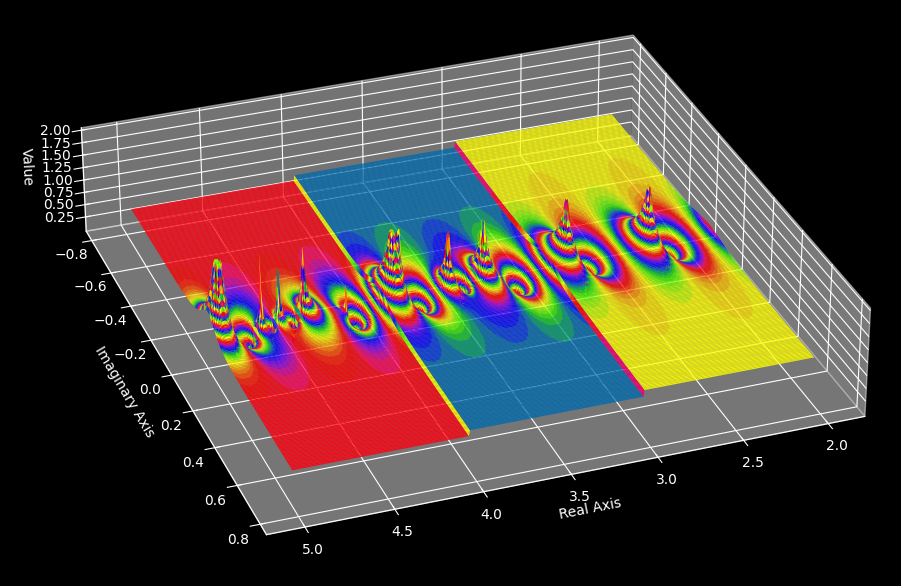
\includegraphics[scale=0.55]{graphs/3D_Complex_Graphs/riesz_tan/HD_Riesz_tan_2_12_n6}
\end{align*}
Figure 29: 3D plot Of E(z) in the complex plane to showcase another angle of E(z) from a closer view.

\newpage
\subsection*{XII. Initial Description of Function H(z)}
We define the Normalized h(z), function $H(z)$ as follows:
\begin{align*}
	I(z) = \frac{\left[\left(|\prod_{n=2}^z\left[\frac{\beta z}{n}\left(1 + |\tan\left(\pi z n\right)|\right)\right]|\right)*\left(|\prod_{n=2}^z\left[\frac{\beta z}{n}\left({\pi z}\prod_{k=2}^z\left(1 - \frac{z^2}{k^2n^2}\right)\right)\right]|\right)\right]^{-m}}{\left[\left(|\prod_{n=2}^z\left[\frac{\beta z}{n}\left(1 + |\tan\left(\pi z n\right)|\right)\right]|\right)*\left(|\prod_{n=2}^z\left[\frac{\beta z}{n}\left({\pi z}\prod_{k=2}^z\left(1 - \frac{z^2}{k^2n^2}\right)\right)\right]|\right)\right]^{-m}!}
\end{align*}

\begin{align*}
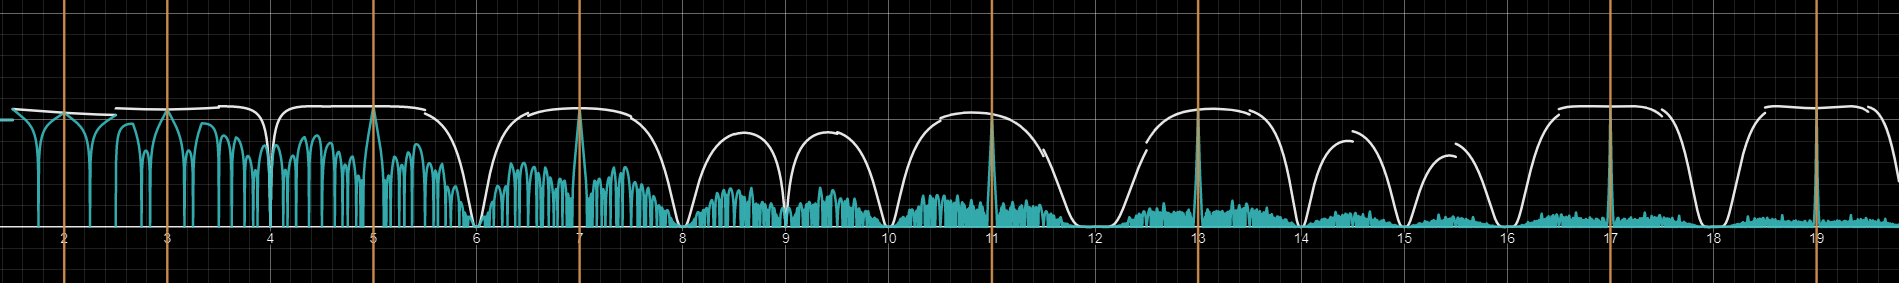
\includegraphics[scale=0.30]{graphs/2D_Real_Graphs/1+tan_prod_xprimefunc}
\end{align*}

The function b(z) allows us to compress l(z) down to the x axis using b(z). The zeros of b(z) are the composite numbers and the non-zero values of b(z) for whole number values of z are prime. this waveform can be combined with the normalized Riesz products to create a new complex wave that is capable of evaluating both the whole numbers and the rational fractions defined by the Riesz products.

\begin{align*}
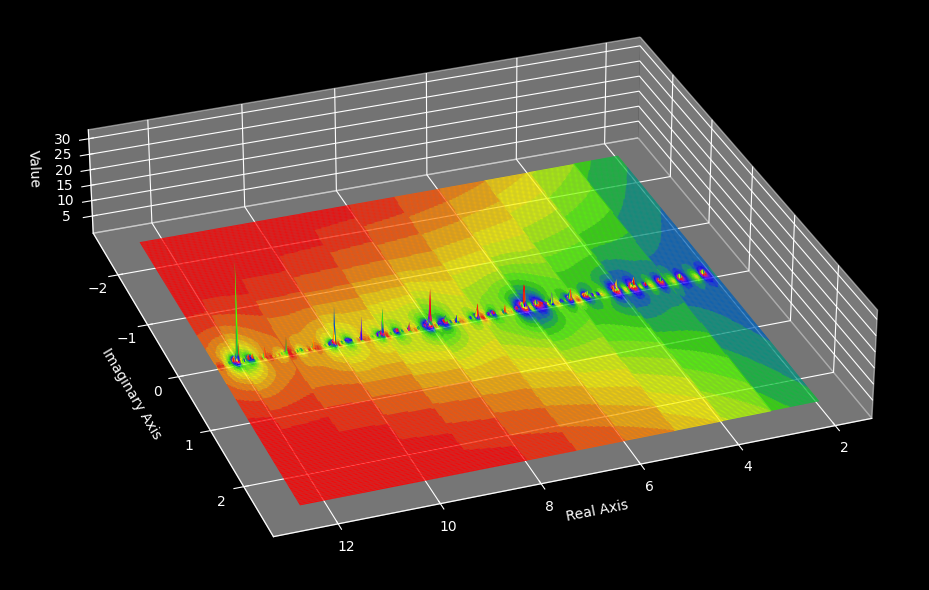
\includegraphics[scale=0.55]{graphs/3D_Complex_Graphs/Riesztan_PrimeFunc/HD_2_12_riesz_tanreversedivisionprimeindc_4}
\end{align*}
Figure 30: 3D plot Of I(z) in the complex plane to showcase the zeros of the combined function.

\newpage
\subsection*{XIII. The Symmetry of Nested Roots: Deriving the First Fundamental Theorem of Analysis through Isomorphisms}

This chapter provides an in-depth examination of the symmetrical isomorphisms inherent in the Nested Roots family. These isomorphisms, characterized by their symmetry and elegance, serve as a derivation of the First Fundamental Theorem of Analysis, thereby offering a novel perspective on these foundational mathematical principles.
\\
Starting with Function j(z) we define the infinite square summation root series, and its equivalent exponent form:
\begin{align*}
j(z) = \sqrt{z + \sqrt{z + \sqrt{z + \ldots}}} = z^{1/2} + z^{1/4} + z^{1/8} + \ldots
\end{align*}

Then by converting the square root series to a factored form we can also formulate the identity:
\begin{align*}
j(z) = \left(z + \left(z + \left(z + \ldots\right)^{1/2}\right)^{1/2}\right)^{1/2} = \ln(\frac{z}{2}\frac{z}{4}\frac{z}{8}\ldots)
\end{align*}

Ultimately leading to the original infinite summation series definition and its equivalent product formula:
\begin{align*}
j(z) = \sum_{n=1}^{\infty} \left[\ln\left(z^{2^{-n})}\right)\right] = ln\left(\prod_{n=1}^{\infty} \left[z^{2^{-n}}\right]\right)
\end{align*}

Now introducing the next function k(z) as another half of the family will show the similarities and differences between j(z) and k(z) and ultimately revealing the First fundamental theorem of Analysis.
\begin{align*}
k(z) = \sqrt{z \cdot \sqrt{z \cdot \sqrt{z \cdot \ldots}}} = z = z^{1/2} * z^{1/4} * z^{1/8} * \ldots
\end{align*}
again, converting the square root chain to a factored form, and forming the exponent of z summation identity:
\begin{align*}
k(z) = \left(z \cdot \left(z \cdot \left(z \cdot \ldots\right)^{1/2}\right)^{1/2}\right)^{1/2} = z^{\frac{1}{2} + \frac{1}{4} + \frac{1}{8} + \ldots}
\end{align*}
Which leads to the original infinite product series definition and its equivalent summation series formula:
\begin{align*}
k(z) = \prod_{n=1}^{\infty} \left[z^{2^{-n}}\right] = z^{(\sidesum{n=1}{\infty}[2^{-n}])}
\end{align*}

\begin{figure}[ht]
\begin{minipage}[b]{0.45\textwidth}
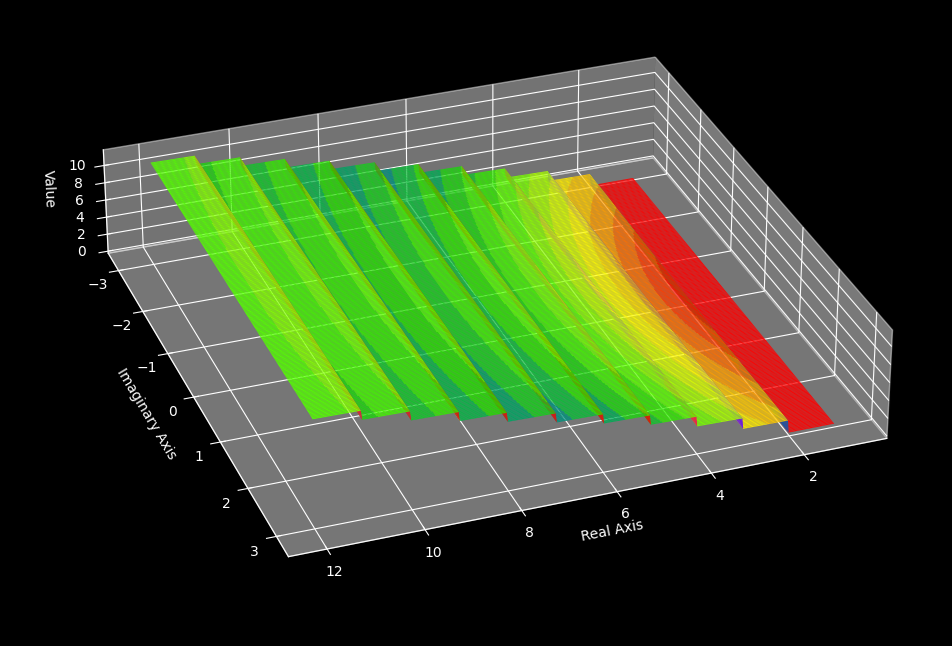
\includegraphics[scale=0.30]{graphs/3D_Complex_Graphs/NestedRoots/Roots_sum}
\caption{3D Complex plot of Nested Roots Sum}
\end{minipage}
\hfill
\begin{minipage}[b]{0.45\textwidth}
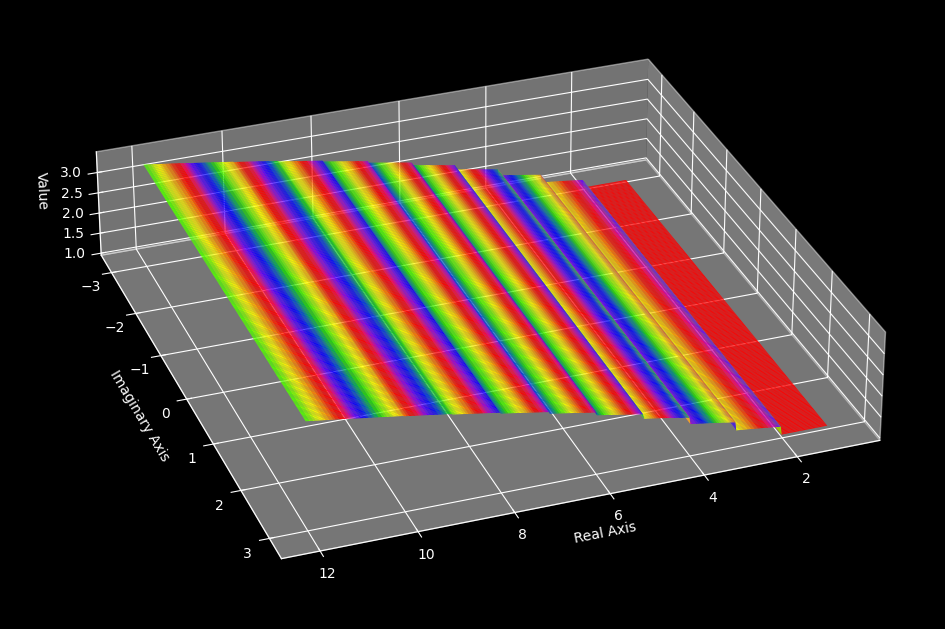
\includegraphics[scale=0.30]{graphs/3D_Complex_Graphs/NestedRoots/Roots_prod}
\caption{3D Complex plot of Nested Roots Product}
\end{minipage}
\end{figure}
From this, the underlying foundation starts to fizzle through, presenting the 4 laws of the First Fundamental theorem of Analysis.

\newpage
The First fundamental theorem of Analysis, which was just derived through the exploration of the Nested Roots family, is an extension of the fundamental theorem of calculus. These laws underpin the entirety of mathematics, and in many cases the 3 identities beyond the first are rarely taught or learned even by math professionals.
\begin{align*}
\SumInt_{a}^{b} f(x) dx = \lim_{n \to \infty}{(\sum_{k=1}^{n} \left[f(x)_{k}\Delta x_{k} \right])}
\end{align*}
The limit definition of the integral above utilizes the same definition we currently use today, however it does introduce a new notation which allows for differentiation from the product integral which currently is defined with poor notation in most texts.

\begin{align*}
\ProdInt_{a}^{b} [ f(x) ]^{dx} = \lim_{n \to \infty}{(\prod_{k=1}^{n} \left[(f(x)_{k})^{\Delta x_{k}} \right])}
\end{align*}
Next is the limit definition of the product integral which follows the same rules as the summation integral however it contains an exponential infinitesimal rather than a coefficient infinitesimal.
\begin{align*}
\ProdInt_{a}^{b} [ f(x) ]^{dx} = e^{\SumInt_{a}^{b} f(x) dx}
\end{align*}
This Formulation provides the 1st way to convert between a product integral and a summation integral.

\begin{align*}
\ln(\prod_{x=a}^{b} [f(x)])= \sum_{x=a}^{b} [\ln(f(x))]
\end{align*}
Finally, this identity allows for the conversion between infinite product series and infinite summation series, note the lack of integration.

Once the revelation becomes clear, it is becomes easier to broaden your perspective on mathematics, and comprehend the duality of infinite summations and infinite products. Ultimately their connection through logarithm rules is beautiful and ironically sensible for exponentiation, and logarithms are two sides of the same coin.

\newpage
\subsection*{XIV. Complex Viete Products, Viete's Paradox, and the Nested Roots Solution}
Chapter XIV will build off of many of the previous ideas presented in this paper. The exploration starts with extending Viete's Products of sin and cos to the complex plane through repeatedly applying the double-angle formula.

Viete's original identity is the following:
\begin{align*}
\frac{2}{\pi} = \prod_{n=1}^{\infty} \cos\left(\frac{\pi}{2^{n+1}}\right)
\end{align*}
Viete formed this relationship from the following infinite series for polygonal circumscribing by comparing the areas of regular polygons with $2^{n}$ and $2^{n+1}$ sides inscribed in a circle.
\begin{align*}
\frac{2}{\pi} = \frac{\sqrt{2}}{2} \cdot \frac{\sqrt{2+\sqrt{2}}}{2} \cdot \frac{\sqrt{2+\sqrt{2+\sqrt{2}}}}{2} \cdot \ldots
\end{align*}
This formula can then be generalized by repeatedly applying the double-angle formula
\begin{align*}
\sin(x) = 2\sin(\frac{x}{2})\cos(\frac{x}{2})
\end{align*}
which leads to a proof by mathematical induction that, for all positive integers n,
\begin{align*}
\sin(x) = 2^{n}\sin(\frac{x}{2^{n}})(\prod_{k=1}^{n} [\cos(\frac{x}{2^{k}})]
\end{align*}
From the previous chapter XIII we can utilize the relationship:
\begin{align*}
\sum_{n=1}^{\infty} 2^{2^{-n}} = \sqrt{2 + \sqrt{2 + \sqrt{\ldots}}}
\end{align*}
and ultimately from Viete's infinite series we can form the relationship:
\begin{align*}
\prod_{k=1}^{\infty} (\frac{\sum_{n=1}^{k} (2^{2^{-n}})}{2}) = \frac{2}{\pi}
\end{align*}

\begin{figure}[ht]
\begin{minipage}[b]{0.45\textwidth}
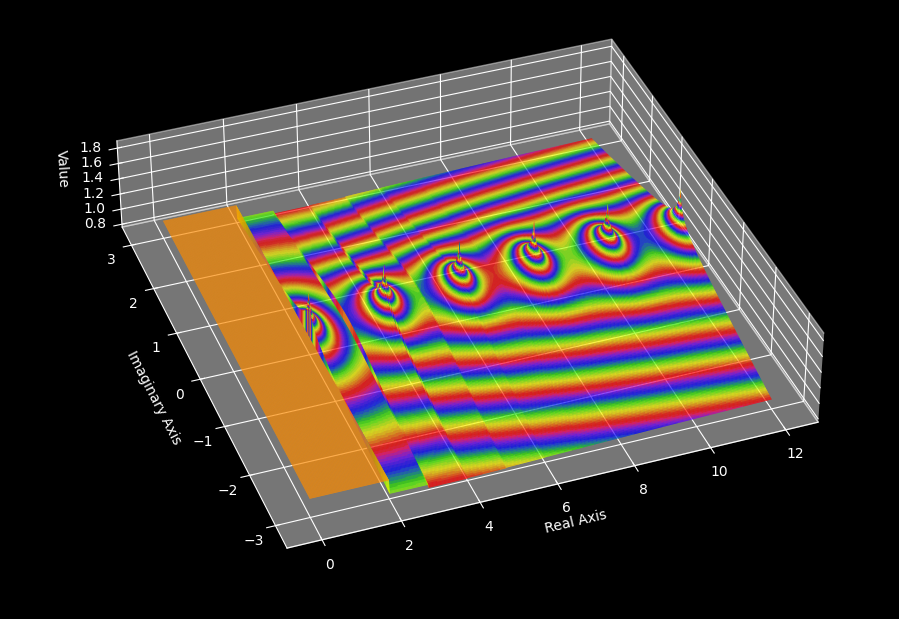
\includegraphics[scale=0.30]{graphs/3D_Complex_Graphs/Viete_cos/Viete_cos_norm_1}
\caption{3D Complex Plot for Viete's product of cos}
\end{minipage}
\hfill
\begin{minipage}[b]{0.45\textwidth}
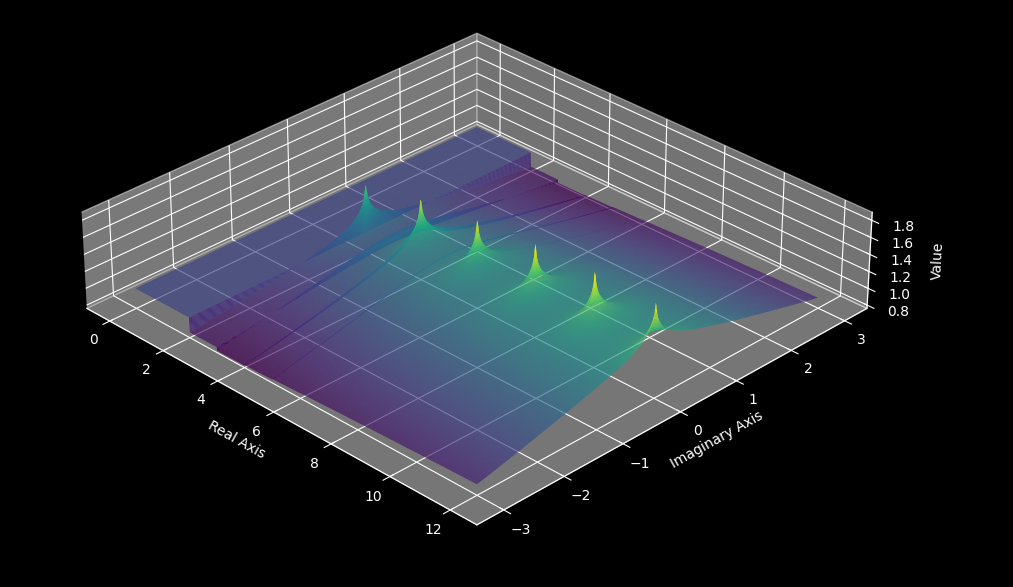
\includegraphics[scale=0.30]{graphs/3D_Complex_Graphs/Viete_cos/Viete_cos_norm_3}
\caption{3D Complex Plot for Viete's product of cos with alternate colorization}
\end{minipage}
\end{figure}

This Plot showcases the zeros of Viete's product as they are spaced in the discrete space of the complex plane.

\newpage
\subsection*{XV. Gamma and Sin Product Identities}
The following section, will give an insight into the intertwined nature of the sin function and the gamma function, by reducing these special functions, down to there core infinite series formulas.
To seed these relationships, we will start with the very well known identity from, (Erica Chang Citation) which goes as follows:

Starting with the key identity relationship between the sine function and the gamma function represented as:
\begin{align*}
sin(\pi z) &= \frac{\pi}{\Gamma\left(z\right) * \Gamma\left(1 - z\right)} \\
\end{align*}
then by taking the product of both sides forming the relationship:
\begin{align*}
\prod_{n=2}^z\left[sin(\frac{\pi * z}{n})\right] &= \prod_{n=2}^z\left[\frac{\pi}{\Gamma\left(\frac{z}{n}\right) * \Gamma\left(1 - \frac{z}{n}\right)}\right] \\
\end{align*}
now taking a look at a different
\begin{align*}
sin(\pi z) &= z\pi * \prod_{k=2}^z\left[1 - \frac{z^2}{k^2}\right] \\
\end{align*}

\begin{align*}
\frac{\pi}{\Gamma\left(z\right) * \Gamma\left(1 - z\right)} &= z\pi * \prod_{k=2}^z\left[1 - \frac{z^2}{k^2}\right] \\
\end{align*}

\begin{align*}
\frac{1}{\Gamma\left(z\right)} &= ze^z^\gamma \prod_{n=2}^z\left[\left(1 + \frac{z^2}{k^2}\right)e^\left(\frac{-z}{n}\right)\right] \\
\end{align*}

\begin{align*}
csc(\pi z) &= \frac{\Gamma\left(z\right) * \Gamma\left(1 - z\right)}{\pi} \\
\end{align*}

\begin{align*}
sin(\pi z) &= \frac{1}{\Gamma\left(z\right)} * \frac{1}{\Gamma\left(- z\right)} * \frac{\pi}{-z} \\
\end{align*}

\begin{align*}
sin(\pi z) &= \frac{\pi}{z} \left(\left[ze^z^\gamma \prod_{n=2}^z \left[\left(1 + \frac{z}{n}\right)e^\frac{-z}{n}\right]\right]\right) * \frac{\pi}{-z} \left(\left[ze^\frac{-z\gamma}{1} \prod_{n=2}^z \left[\left(1 + \frac{-z}{n}\right)e^\frac{z}{n}\right]\right]\right)
\end{align*}

\newpage
\subsection*{XVI. Binary Output Prime Indicator Function H(z)}
The following section demonstrates the combination of many techniques outlined throughout the research of divisor wave analysis, and ultimately will create and develop new methods for prime sieving as well as complex discrete and continuous product functions.

\begin{align*}
H(z) = \left(\frac{|\prod_{n=2}^x \alpha\frac{x}{n}\sin\left(\frac{\pi z}{n}\right)|^{m}}{|\prod_{n=2}^x \alpha\frac{x}{n}\sin\left(\frac{\pi z}{n}\right)|^{m}!}\right)^{\left(\frac{|\prod_{n=2}^x\left[\frac{\beta z}{n}\left({\pi z}\prod_{k=2}^z\left(1 - \frac{z^2}{k^2n^2}\right)\right)\right]|^{m}}{|\prod_{n=2}^x\left[\frac{\beta z}{n}\left({\pi z}\prod_{k=2}^z\left(1 - \frac{z^2}{k^2n^2}\right)\right)\right]|^{m}!}\right)}
\end{align*}

\begin{align*}
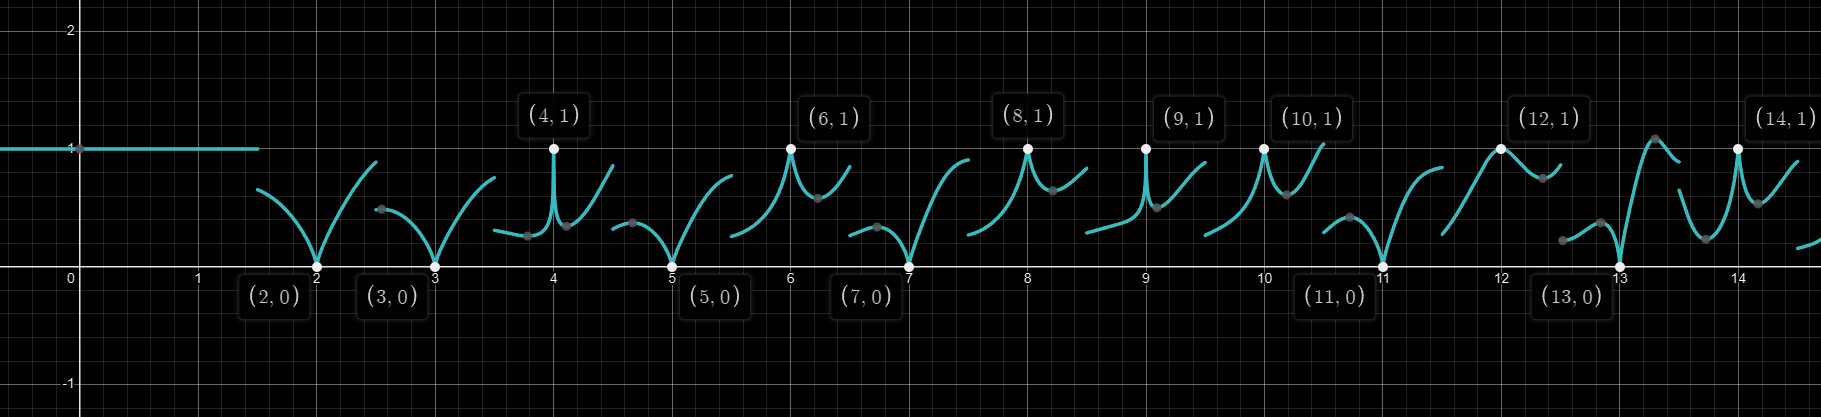
\includegraphics[scale=0.30]{graphs/2D_Real_New/Prime_Indicator_H_normalized_labeled}
\end{align*}
\hspace{8mm}\caption{Figure 35: 2D Graph of $J(x)$ and $H(x)$ showcasing the normalized real zeros of the functions.} \\

The function H(z) combines the previous sieve functions A(z) and B(z) through exponentiation to create a new function. This function H(z) has infinitely many zeros, these zeros correspond with the prime numbers, and for composite numbers H(z) goes to 1. This is a result of B(z) being equal to 0 for composite numbers, and nonzero for prime numbers. Thus A(z) having a zero at all whole numbers each being raised to the power of B(z) where $A(Z)^0 = 1$ and $A(z)^(Non-Zero) = 0$, results in the Binary Output Prime Indicator Function (BOPIF) defined as H(z).

\newpage
\subsection*{XVII. Base 10 Value Output Prime Indicator Function J(z)}
The function J(z) described in the following section is an altered form of H(z), this formula provides the prime numbers in base 10 as the output of the function.

\begin{align*}
J(z) = z * \left(\frac{|\prod_{n=2}^x \alpha\frac{z}{n}\sin\left(\frac{\pi z}{n}\right)|^{m}}{|\prod_{n=2}^x \alpha\frac{z}{n}\sin\left(\frac{\pi z}{n}\right)|^{m}!}\right)^{\left(\left(\frac{|\prod_{n=2}^x \alpha\frac{z}{n}\sin\left(\frac{\pi z}{n}\right)|^{m}}{|\prod_{n=2}^x \alpha\frac{z}{n}\sin\left(\frac{\pi z}{n}\right)|^{m}!}\right)^{\left(\frac{|\prod_{n=2}^x\left[\frac{\beta z}{n}\left({\pi z}\prod_{k=2}^z\left(1 - \frac{z^2}{k^2n^2}\right)\right)\right]|^{m}}{|\prod_{n=2}^x\left[\frac{\beta z}{n}\left({\pi z}\prod_{k=2}^z\left(1 - \frac{z^2}{k^2n^2}\right)\right)\right]|^{m}!}\right)}\right)}
\end{align*}

\begin{align*}
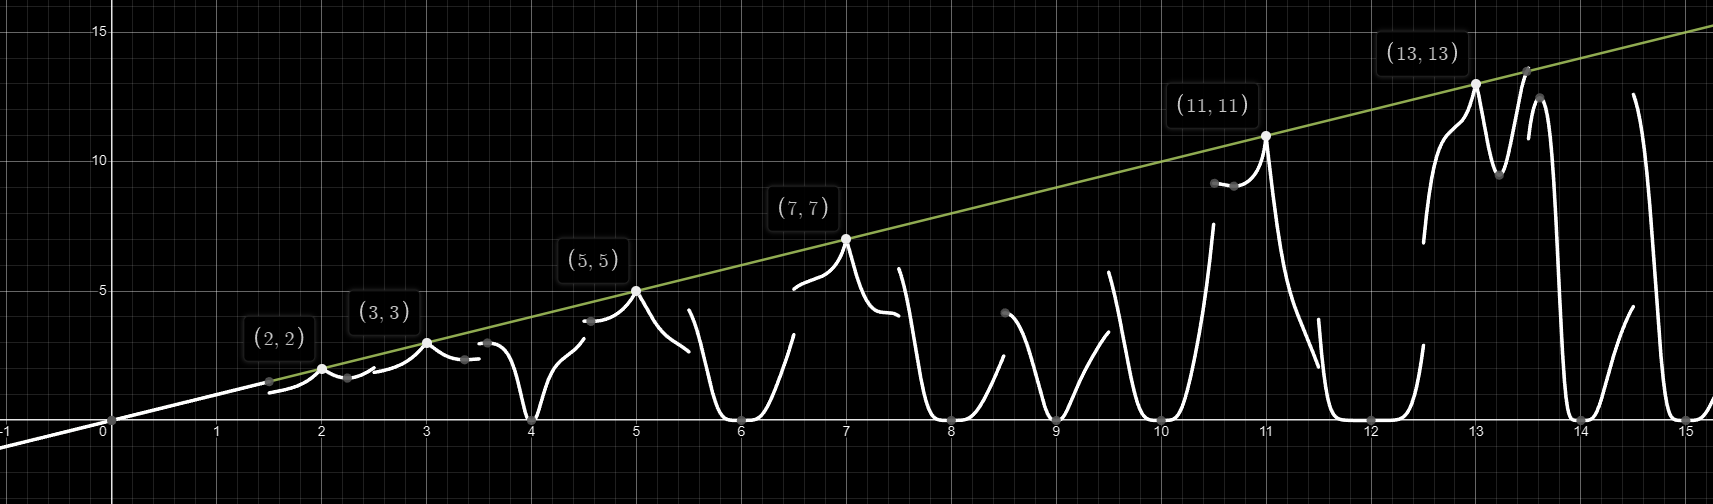
\includegraphics[scale=0.30]{graphs/2D_Real_New/Prime_Indicator_J_normalized}
\end{align*}
\hspace{8mm}\caption{Figure 35: 2D Graph of $J(x)$ and $H(x)$ showcasing the normalized real zeros of the functions.} \\

It can be seen from the plot of J(z) that the function has values of 0 for all composite numbers, and the value of x for all prime numbers, meaning x will always be prime.
this function is put through exponentiation one layer deeper than H(z). When we think of H(z), it is b(z) the set of infinite zeros at composite numbers and non zeros for prime numbers, then being raised to the power of a(z), we have all $0^0=1$ and $0^\left(nonzero\right)$ $=0$, this forced all prime numbers to 0 and all composite numbers to 1. Now A(z) being the set of infinite zeros at all real numbers is the modulation of H(z) to become J(z), J(z) is then $a(z)^0 = 1$  where all prime $z = 0$ and for all composite $z = 1$, then $a(z)^1=0$, this is then multiplied by z and so J(z) is equal to z for all primes, and J(z) is equal to 0 for all composite, the continuous regions between display the discrete product, and how it affects the continuous sin function.

\newpage
\subsection*{XVIII. Euler Product Prime Value Substitution through J(z) as a formulation of \zeta(z)}

\begin{align*}
\zeta(s) = \prod_{n=2}^x \frac{1}{1 - \left( z^{{|\prod_{k=2}^x \sin\left(\frac{\pi z}{k}\right)|}^{|\prod_{k=2}^x \sin\left(\frac{\pi z}{k}\right)|}} \right)^{-s}}
\end{align*}

Through substitution of the primes in the euler product by utilizing the prime indicator function L(z), we can create an alternate product for zeta. This product when e
\newpage
\nocite{*}
\printbibliography
\end{document}
